
\vspace*{1em}
\chapter{Phương Pháp Giải Phương Trình Một Biến}

Trong nhiều bài toán thực tế, việc tìm nghiệm của phương trình một biến đóng vai trò quan trọng trong mô hình hóa và phân tích. Một ví dụ điển hình là mô hình tăng trưởng dân số, trong đó số lượng quần thể $N(t)$ thay đổi theo thời gian $t$ và được mô tả bởi phương trình vi phân:
\[
\frac{dN(t)}{dt} = \lambda N(t),
\]
với nghiệm:
\[
N(t) = N_0 e^{\lambda t},
\]
trong đó $N_0$ là dân số ban đầu và $\lambda$ là tỷ lệ sinh.

\begin{center}
\begin{tikzpicture}
\begin{axis}[
    width=10cm,
    height=7cm,
    xlabel={Tỷ lệ sinh $\lambda$},
    ylabel={Dân số (nghìn)},
    xmin=0, xmax=1.2,
    ymin=1000, ymax=3200,
    domain=0:1,
    samples=100,
    axis lines=middle,
    xtick={0,0.5,1},
    ytick={1000,1435,1564,2000,3000},
    yticklabels={1000,1435,1564,2000,3000},
    xlabel style={at={(axis description cs:1,0)},anchor=west},
    ylabel style={at={(axis description cs:0,1)},anchor=south},
]
% Vẽ đường cong N(λ) = 1000 e^x + (435/x)(e^x - 1)
\addplot[blue, thick] {1000*exp(x) + (435/x)*(exp(x)-1)};
% Ghi chú công thức
\node at (axis cs:0.6,2200) {$N(\lambda)=1000e^{\lambda}+\dfrac{435}{\lambda}(e^{\lambda}-1)$};
% Đường ngang tại 1564 và 1435
\draw[dashed] (axis cs:0,1564) -- (axis cs:1,1564);
\draw[dashed] (axis cs:0,1435) -- (axis cs:1,1435);
\end{axis}
\end{tikzpicture}
\end{center}


Khi có thêm yếu tố nhập cư với tốc độ không đổi $v$, phương trình trở thành:
\[
\frac{dN(t)}{dt} = \lambda N(t) + v,
\]
với nghiệm:
\[
N(t) = N_0 e^{\lambda t} + \frac{v}{\lambda}(e^{\lambda t} - 1).
\]

Trong thực tế, để xác định $\lambda$ từ dữ liệu quan sát, ta phải giải phương trình phi tuyến:
\[
1{,}564{,}000 = 1{,}000{,}000 e^{\lambda} + \frac{435{,}000}{\lambda}(e^{\lambda} - 1).
\]

Phương trình này không thể giải tường minh, do đó cần sử dụng các phương pháp số như \textit{phương pháp chia đôi}, \textit{lặp điểm cố định} hoặc \textit{phương pháp Newton} để tìm nghiệm gần đúng. Đây chính là lý do các kỹ thuật giải phương trình một biến trở thành công cụ thiết yếu trong phân tích số và ứng dụng thực tế.


\section{Phương pháp Chia Đôi (Bisection Method)}
\label{sec:bisection_method}

Trong chương này, chúng ta xem xét một trong những vấn đề cơ bản nhất của xấp xỉ số,
đó là \textit{bài toán tìm nghiệm}. Bài toán liên quan đến việc tìm một \textit{nghiệm}
của phương trình dạng $f(x)=0$ đối với một hàm $f$ cho trước. Một nghiệm của phương trình này
còn được gọi là một \textit{zero} của hàm $f$.

Bài toán tìm nghiệm xấp xỉ đã được biết đến từ thời Babylon cổ đại. Ví dụ,
họ đã xấp xỉ $\sqrt{2}$ đến độ chính xác $10^{-5}$. 

%---------------------------------------------------------
\subsection{Kỹ thuật Chia Đôi}
\label{subsec:bisection_technique}

Kỹ thuật này dựa trên \textit{Định lý Giá trị Trung gian (Intermediate Value Theorem)}
và được gọi là \textit{phương pháp chia đôi (bisection)} hoặc \textit{binary-search}.

Giả sử $f$ liên tục trên khoảng $[a,b]$, và $f(a)f(b) < 0$, khi đó tồn tại $p \in (a,b)$
sao cho $f(p)=0$.

Đặt $a_1=a$, $b_1=b$ và
\[
p_1 = \frac{a_1 + b_1}{2}.
\]

\begin{itemize}
    \item Nếu $f(p_1)=0$, khi đó nghiệm $p=p_1$.
    \item Nếu $f(p_1) \neq 0$:
        \begin{itemize}
            \item Nếu $f(a_1)$ và $f(p_1)$ cùng dấu, đặt $a_2=p_1$, $b_2=b_1$.
            \item Nếu trái dấu, đặt $a_2=a_1$, $b_2=p_1$.
        \end{itemize}
\end{itemize}

Tiếp tục quy trình đối với khoảng $[a_2,b_2]$.

\begin{figure}[!h]
\centering
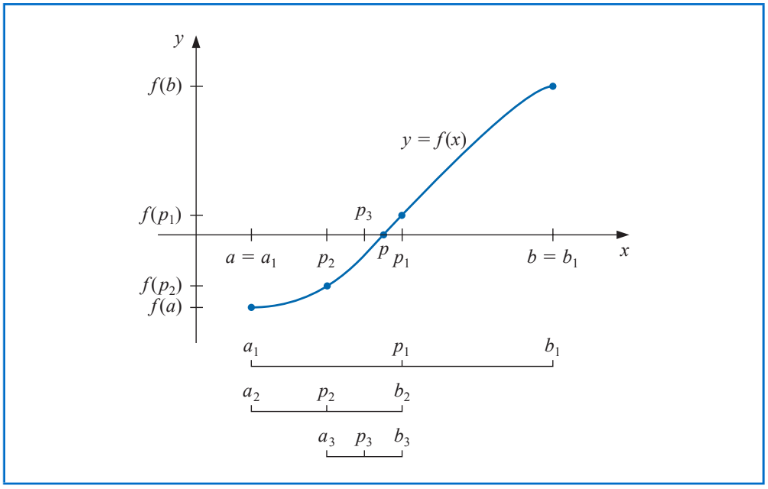
\includegraphics[width=0.65\linewidth]{figures/bisect_diagram_placeholder.png}
\caption{Minh họa phương pháp chia đôi.}
\label{fig:bisection_figure1}
\end{figure}

%---------------------------------------------------------
\subsection{Thuật toán Chia Đôi}
\label{subsec:bisection_algorithm}

\begin{algorithm}
\caption{Thuật toán Chia Đôi}
\label{alg:bisection}
\begin{algorithmic}[1]
\Require $a,b$ sao cho $f(a)f(b) < 0$, sai số $TOL$, số lặp tối đa $N_0$
\Ensure Nghiệm xấp xỉ $p$
\State $i \gets 1$
\State $FA \gets f(a)$
\While {$i \le N_0$}
    \State $p \gets a + \frac{b-a}{2}$
    \State $FP \gets f(p)$
    \If {$FP = 0$ or $\frac{b-a}{2} < TOL$}
        \Return $p$
    \EndIf
    \State $i \gets i+1$
    \If {$FA \cdot FP > 0$}
        \State $a \gets p$
        \State $FA \gets FP$
    \Else
        \State $b \gets p$
    \EndIf
\EndWhile
\Return {``Thất bại sau $N_0$ lặp.''}
\end{algorithmic}
\end{algorithm}

\subsection*{Các tiêu chí dừng bổ sung}
\label{subsec:additional_stopping}

Trong Bước~4 của Thuật toán~\ref{alg:bisection}, hoặc trong bất kỳ kỹ thuật lặp nào
được trình bày trong chương này, ta có thể áp dụng các tiêu chí dừng thay thế.
Ví dụ, ta có thể chọn một sai số $\varepsilon > 0$ và sinh ra dãy
$p_1, p_2, \dots, p_n$ cho đến khi thỏa mãn một trong các điều kiện sau:

\begin{align}
|p_n - p_{n-1}| &< \varepsilon, \label{eq:stop_a}\\[6pt]
\frac{|p_n - p_{n-1}|}{|p_n|} &< \varepsilon, \quad p_n \neq 0, \label{eq:stop_b}\\[6pt]
|f(p_n)| &< \varepsilon. \label{eq:stop_c}
\end{align}

Tuy nhiên, trong thực tế, một số khó khăn có thể phát sinh khi sử dụng riêng lẻ
bất kỳ tiêu chí dừng nào ở trên. Chẳng hạn, tồn tại các dãy $\{p_n\}_{n=1}^{\infty}$
mà sai khác $p_n - p_{n-1}$ tiến dần về 0, nhưng bản thân dãy lại \emph{diverge}
(không hội tụ). (Xem Bài tập~\ref{ex:exercise17}.) Ngoài ra, cũng có thể xảy ra trường hợp
giá trị $f(p_n)$ rất nhỏ trong khi khoảng cách $p_n$ đến nghiệm thực sự $p$ vẫn khác biệt đáng kể.

Khi không có thông tin bổ sung về độ lớn tuyệt đối hoặc tương đối của $p$, tiêu chí
tương đối \eqref{eq:stop_b} thường được xem là tốt hơn, vì nó gần nhất với ý nghĩa
sai số tương đối trong thực tế tính toán.

\subsection*{Giới hạn số vòng lặp}
\label{subsec:max_iterations}

Khi sử dụng máy tính để tạo xấp xỉ, việc đặt ra \textit{số vòng lặp tối đa} (iteration limit)
là một thực hành tốt. Điều này loại bỏ khả năng rơi vào vòng lặp vô hạn do sai sót trong việc
kiểm tra điều kiện dừng hoặc lập trình sai. Điều này đã được thực hiện trong Bước~2 của
Thuật toán~\ref{alg:bisection}, nơi giá trị $N_0$ được thiết lập và thủ tục sẽ dừng nếu
$i > N_0$.

\subsection*{Lựa chọn khoảng ban đầu}
\label{subsec:initial_interval}

Lưu ý rằng để bắt đầu Thuật toán Chia Đôi, đoạn $[a,b]$ phải thỏa $f(a)f(b) < 0$.
Ở mỗi bước, độ dài của đoạn chứa nghiệm giảm đi một hệ số $2$; do đó, việc chọn
đoạn ban đầu càng nhỏ càng tốt là điều có lợi.

Ví dụ, xét hàm:
\[
f(x) = 2x^3 - x^2 + x - 1.
\]

Ta có:
\[
f(-4)\cdot f(4) < 0
\quad\text{và}\quad
f(0)\cdot f(1) < 0.
\]

Do đó, có thể bắt đầu Thuật toán Chia Đôi trên đoạn $[-4,4]$ hoặc trên $[0,1]$.
Nếu xét đoạn $[0,1]$ thay vì $[-4,4]$, số vòng lặp cần thiết để đạt cùng độ chính xác
sẽ giảm đi khoảng $\log_2(8) = 3$ bước (tương ứng việc rút nhỏ đoạn ban đầu).

\label{subsec:example1}

\begin{example}
Xét phương trình
\[
f(x) = x^3 + 4x^2 - 10 = 0.
\]
Chứng minh rằng phương trình có nghiệm trong khoảng $[1,2]$ và sử dụng
phương pháp chia đôi (Bisection) để tìm nghiệm xấp xỉ với độ chính xác
ít nhất $10^{-4}$.
\end{example}

\paragraph*{Bước 1: Chứng minh tồn tại nghiệm.}
Ta có
\[
f(1) = 1^3 + 4(1)^2 - 10 = -5 < 0,
\qquad
f(2) = 2^3 + 4(2)^2 - 10 = 14 > 0.
\]
Vì $f(1)\cdot f(2) < 0$ nên theo Định lý Giá trị Trung gian,
tồn tại ít nhất một nghiệm $p \in (1,2)$.

\paragraph*{Bước 2: Áp dụng phương pháp chia đôi.}
Ta bắt đầu với $a_1 = 1$, $b_1 = 2$ và tính trung điểm
\[
p_1 = \frac{a_1 + b_1}{2} = 1.5.
\]

Sau đó ta kiểm tra dấu $f(a_n)$ và $f(p_n)$
để xác định khoảng con chứa nghiệm tại mỗi bước.

\paragraph*{Bảng tính lặp.}

\begin{table}[!h]
\centering
\caption{Các bước lặp của phương pháp chia đôi cho Ví dụ~\ref{subsec:example1}.}
\label{tab:example1-bisection}
\begin{tabular}{cccc}
\toprule
$n$ & $a_n$ & $b_n$ & $p_n$ \\
\midrule
1  & 1.0000       & 2.0000       & 1.5000 \\
2  & 1.0000       & 1.5000       & 1.2500 \\
3  & 1.2500       & 1.5000       & 1.3750 \\
4  & 1.2500       & 1.3750       & 1.3125 \\
5  & 1.3125       & 1.3750       & 1.34375 \\
6  & 1.34375      & 1.3750       & 1.359375 \\
7  & 1.359375     & 1.3750       & 1.3671875 \\
8  & 1.359375     & 1.3671875    & 1.36328125 \\
9  & 1.359375     & 1.36328125   & 1.361328125 \\
10 & 1.361328125  & 1.36328125   & 1.3623046875 \\
11 & 1.361328125  & 1.3623046875 & 1.36181640625 \\
12 & 1.36181640625 & 1.3623046875 & 1.362060546875 \\
13 & 1.36181640625 & 1.362060546875 & 1.3619384765625 \\
\bottomrule
\end{tabular}
\end{table}

\paragraph*{Bước 3: Kiểm tra tiêu chí dừng.}
Độ dài khoảng sau $n$ bước bằng
\[
b_n - a_n = \frac{2 - 1}{2^{n-1}} = \frac{1}{2^{n-1}}.
\]
Sai số tuyệt đối được chặn bởi
\[
|p - p_n| \le \frac{b_n - a_n}{2} = \frac{1}{2^n}.
\]

Tại $n = 13$,
\[
\frac{1}{2^{13}} = \frac{1}{8192} \approx 1.2207\times10^{-4} < 10^{-4},
\]
do đó sai số đã nhỏ hơn yêu cầu.

\paragraph*{Kết luận.}
Phương trình $f(x)=0$ có nghiệm trong $(1,2)$ và phương pháp chia đôi
cho xấp xỉ nghiệm:
\[
p \approx 1.36194,
\]
với sai số nhỏ hơn $10^{-4}$.

\begin{theorem}
\label{thm:bisection_convergence}
Giả sử $f$ liên tục trên đoạn $[a,b]$ và $f(a)\cdot f(b) < 0$. Phương pháp Chia Đôi
(Bisection) sinh ra dãy $\{p_n\}_{n=1}^{\infty}$ xấp xỉ nghiệm $p$ của phương trình
$f(x)=0$ sao cho
\[
|p_n - p| \le \frac{b - a}{2^n}, \qquad n \ge 1.
\]
\end{theorem}

\begin{proof}
Với mỗi $n \ge 1$, do phương pháp chia đôi bảo toàn dấu theo Định lý Giá trị Trung gian,
nghiệm $p$ luôn nằm trong khoảng $(a_n,b_n)$, nơi $b_n - a_n = \dfrac{1}{2^{\,n-1}}(b-a)$.

Vì $p_n$ là trung điểm khoảng $[a_n,b_n]$, nên
\[
|p_n - p| \le \frac{1}{2}(b_n - a_n) = \frac{b-a}{2^n}.
\]

Do đó
\[
|p_{n} - p| \le \frac{b-a}{2^n}.
\]

Từ đây ta suy ra dãy $\{p_n\}$ hội tụ về $p$ với tốc độ hội tụ
\[
p_n = p + \mathcal{O}\!\left(\frac{1}{2^n}\right).
\]
\end{proof}

\noindent
Lưu ý rằng định lý trên chỉ đưa ra một \emph{chặn trên} cho sai số xấp xỉ,
và trong thực tế chặn này có thể khá bảo thủ. Ví dụ, trong
Ví dụ~\ref{subsec:example1}, ta chỉ đảm bảo rằng
\[
|p - p_{9}| \le \frac{2-1}{2^9} = \frac{1}{512} \approx 2\times 10^{-3},
\]
nhưng sai số thực tế nhỏ hơn nhiều:
\[
|\,p - p_{9}\,| = |\,1.365230013 - 1.365234375\,|
    \approx 4.4\times 10^{-6}.
\]










\section{Phương pháp Lặp Điểm Cố Định (Fixed-Point Iteration)}
\label{sec:fixed_point_iteration}

Một \emph{điểm cố định} (fixed point) của một hàm là một số mà tại đó
giá trị của hàm không thay đổi sau khi được áp dụng.

\begin{definition}
\label{def:fixed_point}
Một số $p$ được gọi là \emph{điểm cố định} của hàm $g$ nếu
\[
g(p) = p.
\]
\end{definition}

Trong mục này, chúng ta xem xét bài toán tìm nghiệm của các hàm dưới dạng điểm cố định,
và mối liên hệ giữa bài toán điểm cố định và bài toán tìm nghiệm dạng $f(x)=0$.

Trên thực tế, hai lớp bài toán này là \emph{tương đương} theo các ý sau:

\begin{itemize}
    \item Nếu ta có bài toán tìm nghiệm $f(p)=0$, ta có thể xây dựng
    một hàm $g$ sao cho $p$ là điểm cố định:
    \[
    g(x) = x - f(x)
    \qquad \text{hoặc} \qquad
    g(x) = x + 3f(x),
    \]
    hay nhiều dạng khác.
    \item Ngược lại, nếu một hàm $g$ có điểm cố định $p$, thì hàm
    \[
    f(x) = x - g(x)
    \]
    sẽ có nghiệm tại $p$.
\end{itemize}

Như vậy, thay vì giải phương trình $f(x)=0$, ta có thể chuyển sang bài toán
tìm điểm cố định $g(x)=x$ — đôi khi đơn giản và dễ phân tích hơn.

\begin{remark}
Mặc dù các kỹ thuật tìm nghiệm thường được trình bày dưới dạng $f(x)=0$,
dạng điểm cố định $g(x)=x$ giúp xây dựng các phương pháp lặp mạnh và tinh tế hơn.
Ý tưởng nền tảng được hình thức hóa bởi nhà toán học người Hà Lan
L. E. J. Brouwer (1882–1962) vào đầu thế kỷ XX.
\end{remark}

Để sử dụng dạng này hiệu quả, chúng ta cần:
\begin{enumerate}
    \item Nhận biết khi nào một hàm $g$ có điểm cố định;
    \item Xem xét cách xấp xỉ điểm cố định $p$ với độ chính xác chỉ định.
\end{enumerate}

\begin{theorem}
\label{thm:fixed_point_existence_uniqueness}
Giả sử $g$ là hàm liên tục trên đoạn $[a,b]$ và $g(x) \in [a,b]$ với mọi $x \in [a,b]$.
Khi đó:
\begin{enumerate}
    \item Hàm $g$ tồn tại ít nhất một điểm cố định trong $[a,b]$.
    \item Nếu, thêm vào đó, $g$ khả vi trên $(a,b)$ và tồn tại hằng số dương $k<1$
    sao cho
    \[
    |g'(x)| \le k, \quad \forall x \in (a,b),
    \]
    thì điểm cố định trên là \emph{duy nhất} trong $[a,b]$.
\end{enumerate}
\end{theorem}

\begin{figure}[!h]
\centering
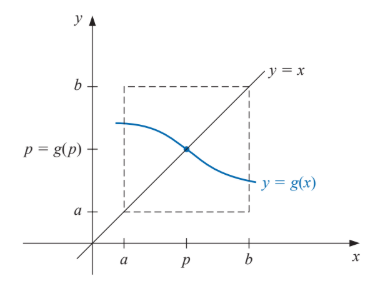
\includegraphics[width=0.6\linewidth]{figures/fixed_point_diagram_placeholder.png}
\caption{Minh họa điểm cố định của $g(x)$ trong $[a,b]$.}
\label{fig:fixed_point_figure}
\end{figure}

\begin{proof}

\textbf{(i)} Nếu $g(a) = a$ hoặc $g(b) = b$, ta đã có điểm cố định tại đầu mút.
Ngược lại, nếu
\[
g(a) > a \quad \text{và} \quad g(b) < b,
\]
xét hàm
\[
h(x) = g(x) - x.
\]
Do $g(x) \in [a,b]$, ta có $h(a) = g(a) - a > 0$ và $h(b) = g(b) - b < 0$.
Vì $h$ liên tục trên $[a,b]$, Định lý Giá trị Trung gian (IVT) suy ra tồn tại $p \in (a,b)$ sao cho
\[
h(p) = 0 \quad \Longleftrightarrow \quad g(p) = p.
\]
Do đó, $p$ là điểm cố định.

\bigskip
\textbf{(ii)} Giả sử tồn tại thêm điều kiện $|g'(x)| \le k < 1$ trên $(a,b)$.
Giả sử $p$ và $q$ đều là các điểm cố định trong $[a,b]$:
\[
g(p) = p, \qquad g(q) = q.
\]

Nếu $p \neq q$, áp dụng Định lý Giá trị Trung bình (MVT), tồn tại $\xi \in (a,b)$ sao cho
\[
\frac{g(p) - g(q)}{p - q} = g'(\xi).
\]
Do đó,
\[
|p - q|
= |g(p) - g(q)|
= |g'(\xi)|\,|p - q|
\le k\,|p - q|.
\]

Vì $0 \le k < 1$, biểu thức trên chỉ có thể xảy ra nếu $|p - q| = 0$, tức là $p=q$.

Suy ra điểm cố định là duy nhất.

\end{proof}

\subsection{Phương pháp Lặp Điểm Cố Định (Fixed-Point Iteration)}
\label{subsec:fixed_point_iteration}

Xét phương trình $x = g(x)$, trong đó ta không thể giải tường minh được nghiệm $p$.
Tuy nhiên, ta có thể tìm \emph{xấp xỉ} của điểm cố định $p$ đến một độ chính xác tùy ý
thông qua lặp điểm cố định.

Để xấp xỉ điểm cố định của hàm $g$, ta chọn giá trị khởi tạo $p_0$ và sinh dãy
$\{p_n\}_{n=0}^{\infty}$ bằng quy luật:
\[
p_n = g(p_{n-1}), \qquad n \ge 1.
\]

Nếu dãy này hội tụ đến $p$ và $g$ liên tục, ta có:
\[
p = \lim_{n\to\infty} p_n = \lim_{n\to\infty} g(p_{n-1})
  = g\!\left(\lim_{n\to\infty} p_{n-1}\right) = g(p).
\]
Như vậy $p$ là nghiệm của $x = g(x)$, hay tương đương là nghiệm của $f(x) = x - g(x) = 0$.

Kỹ thuật này được gọi là \textbf{phương pháp lặp điểm cố định} (fixed-point iteration),
hoặc \textbf{functional iteration}.

%-------------------------------------------------------------
\begin{figure}[!h]
\centering
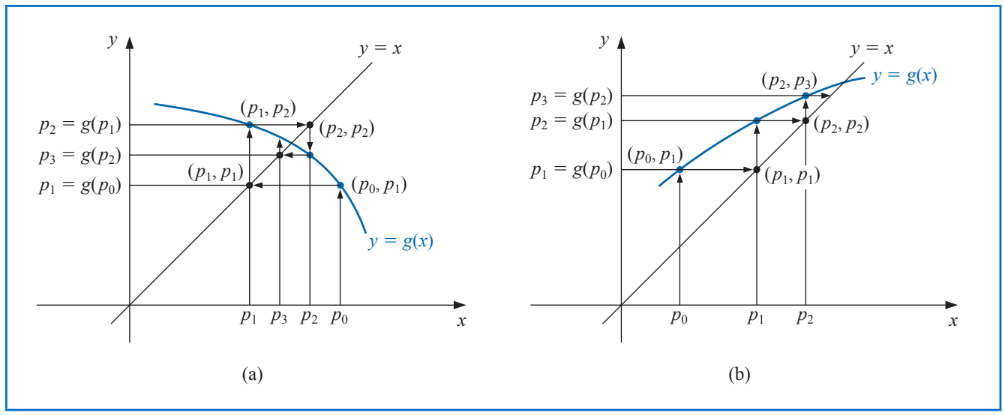
\includegraphics[width=0.8\linewidth]{figures/fixed_point_iteration_placeholder.png}
\caption{Minh họa quá trình lặp điểm cố định: (a) hội tụ chậm, (b) hội tụ nhanh.}
\label{fig:fixed_point_iteration}
\end{figure}

%-------------------------------------------------------------
\begin{algorithm}[!h]
\caption{Fixed-Point Iteration}
\label{alg:fixed_point_iteration}
\begin{algorithmic}[1]
\State Chọn xấp xỉ ban đầu $p_0$; ngưỡng sai số $\text{TOL}$; số lặp tối đa $N_0$.
\State $i \gets 1$.
\While{$i \le N_0$}
    \State $p \gets g(p_0)$ \hfill \% tính giá trị lặp mới
    \If{$|p - p_0| < \text{TOL}$}
        \State \Return $p$ \hfill \% thuật toán thành công
    \EndIf
    \State $i \gets i + 1$
    \State $p_0 \gets p$ \hfill \% cập nhật giá trị lặp
\EndWhile
\State \Return \texttt{"Thất bại: vượt quá $N_0$ vòng lặp."}
\end{algorithmic}
\end{algorithm}


%-------------------------------------------------------------
\subsubsection*{Ví dụ minh họa}

Xét phương trình
\[
x^3 + 4x^2 - 10 = 0,
\]
phương trình này có nghiệm duy nhất trong $[1,2]$ (xem lại Ví dụ~\ref{subsec:example1}).

Ta có thể viết lại phương trình về dạng điểm cố định $x = g(x)$ theo nhiều cách.
Ví dụ:
\begin{align*}
\text{(a)}\;& x = g_1(x) = x - x^3 - 4x^2 + 10,\\
\text{(b)}\;& x = g_2(x) = \sqrt{10/x - 4x},\\
\text{(c)}\;& x = g_3(x) = \tfrac{1}{2}\sqrt{10 - x^3},\\
\text{(d)}\;& x = g_4(x) = \sqrt{\tfrac{10}{4 + x}},\\
\text{(e)}\;& x = g_5(x) = x - \frac{x^3 + 4x^2 - 10}{3x^2 + 8x}.
\end{align*}

Giả sử chọn $p_0 = 1.5$, ta thực hiện thuật toán~\ref{alg:fixed_point_iteration} cho mỗi hàm $g_i$.

\begin{table}[!h]
\centering
\caption{Kết quả của phương pháp lặp điểm cố định cho năm dạng $g_i$.}
\label{tab:fixed_point_results}
\begin{tabular}{c|ccccc}
\toprule
$n$ & (a) & (b) & (c) & (d) & (e) \\
\midrule
0  & 1.5 & 1.5 & 1.5 & 1.5 & 1.5 \\
1  & -0.875 & 0.8165 & 1.28695 & 1.34840 & 1.37333 \\
2  & 6.732 & 2.9969 & 1.40254 & 1.36737 & 1.36521 \\
3  & -469.7 & $\sqrt{-8.65}$ & 1.34546 & 1.36496 & 1.36523 \\
4  & $1.03\times10^8$ & --- & 1.37517 & 1.36526 & 1.36523 \\
5  & --- & --- & 1.36009 & 1.36522 & 1.36523 \\
10 & --- & --- & 1.36478 & 1.36523 & 1.36523 \\
15 & --- & --- & 1.36522 & 1.36523 & 1.36523 \\
20 & --- & --- & 1.36523 & 1.36523 & 1.36523 \\
25 & --- & --- & 1.36523 & 1.36523 & 1.36523 \\
30 & --- & --- & 1.36523 & 1.36523 & 1.36523 \\
\bottomrule
\end{tabular}
\end{table}

Nghiệm thật (so sánh từ Ví dụ~\ref{subsec:example1}) là:
\[
p = 1.365230013.
\]
Ta thấy các lựa chọn (c), (d), và (e) hội tụ nhanh đến nghiệm thật, trong khi (a) phân kỳ
và (b) trở nên không xác định (do biểu thức căn của số âm).

\begin{remark}
Phương pháp chia đôi yêu cầu 27 vòng lặp để đạt cùng độ chính xác $10^{-4}$,
trong khi các biến thể điểm cố định như (c)–(e) chỉ cần chưa đến 10 vòng lặp.
Điều này minh họa sức mạnh của việc chọn dạng $g(x)$ thích hợp.
\end{remark}

\begin{theorem}[Định lý điểm cố định]
\label{thm:fixed_point_theorem}
Giả sử $g \in C[a,b]$ và $g(x)\in[a,b]$ với mọi $x\in[a,b]$.  
Giả sử thêm rằng $g'(x)$ tồn tại trên $(a,b)$ và tồn tại hằng số $k$ với $0<k<1$ sao cho
\[
|g'(x)| \le k, \qquad \forall x \in (a,b).
\]
Khi đó, với mọi giá trị khởi tạo $p_0 \in [a,b]$, dãy được xác định bởi
\[
p_n = g(p_{n-1}), \qquad n \ge 1,
\]
hội tụ đến điểm cố định duy nhất $p \in [a,b]$ của $g$.
\end{theorem}

\begin{proof}
Theo Định lý~\ref{thm:fixed_point_existence_uniqueness}, $g$ có đúng một điểm cố định $p$ sao cho $g(p)=p$.  
Với mỗi $n\ge1$, áp dụng Định lý Giá trị Trung bình (Mean Value Theorem) cho $g$ trên khoảng $(p_{n-1},p)$, tồn tại $\xi_n \in (a,b)$ sao cho
\[
|p_n - p|
  = |g(p_{n-1}) - g(p)|
  = |g'(\xi_n)|\,|p_{n-1}-p|
  \le k\,|p_{n-1}-p|.
\]
Suy ra theo quy nạp
\[
|p_n - p| \le k^n |p_0 - p|.
\tag{*}\label{eq:fixedpoint_error}
\]
Vì $0<k<1$, ta có $\lim_{n\to\infty} k^n = 0$, do đó
\[
\lim_{n\to\infty} |p_n - p| = 0,
\]
nghĩa là $\{p_n\}$ hội tụ đến $p$.
\end{proof}

\begin{corollary}[Sai số của phép lặp điểm cố định]
\label{cor:fixed_point_error}
Nếu $g$ thỏa các giả thiết của Định lý~\ref{thm:fixed_point_theorem}, thì sai số khi dùng $p_n$ để xấp xỉ $p$ được chặn bởi
\begin{align}
|p_n - p| &\le k^n \max\{|p_0 - a|,\;|b - p_0|\}, \label{eq:fixedpoint_bound1}\\[3pt]
|p_n - p| &\le \frac{k^n}{1-k}\,|p_1 - p_0|, \qquad n \ge 1. \label{eq:fixedpoint_bound2}
\end{align}
\end{corollary}

\begin{proof}
Vì $p\in[a,b]$, từ bất đẳng thức~\eqref{eq:fixedpoint_error} suy ra
\[
|p_n - p| \le k^n |p_0 - p| \le k^n \max\{|p_0 - a|,\,|b - p_0|\},
\]
cho~\eqref{eq:fixedpoint_bound1}.  

Tiếp theo, theo chứng minh của Định lý~\ref{thm:fixed_point_theorem},
\[
|p_{n+1} - p_n| = |g(p_n) - g(p_{n-1})|
 \le k\,|p_n - p_{n-1}|.
\]
Suy ra bằng quy nạp
\[
|p_{n+j} - p_{n+j-1}| \le k^{j-1}|p_1 - p_0|.
\]
Tổng các sai số vi phân này cho $m>n\ge1$:
\[
|p_m - p_n|
  \le \sum_{i=n}^{m-1}|p_{i+1}-p_i|
  \le |p_1 - p_0|\!\!\sum_{i=n}^{m-1}\!k^i
  \le \frac{k^n}{1-k}|p_1 - p_0|.
\]
Cho $m\!\to\!\infty$ ta được~\eqref{eq:fixedpoint_bound2}.
\end{proof}

\subsubsection*{Phân tích các hàm lặp điểm cố định}

Xét lại các hàm $g_1, g_2, g_3, g_4, g_5$ được sử dụng trong ví dụ trước, theo định lý điểm cố định~\ref{thm:fixed_point_theorem} và hệ quả~\ref{cor:fixed_point_error}.

\paragraph*{(a) Hàm $g_1(x) = x - x^3 - 4x^2 + 10$}

Ta có $g_1(1) = 6$ và $g_1(2) = -12$, do đó $g_1$ không ánh xạ đoạn $[1,2]$ vào chính nó.  
Thêm nữa, $g_1'(x) = 1 - 3x^2 - 8x$, nên $|g_1'(x)| > 1$ với mọi $x \in [1,2]$.  
Theo định lý điểm cố định, điều kiện này không đảm bảo hội tụ — vì vậy không có lý do để mong đợi phương pháp này hội tụ.

\paragraph*{(b) Hàm $g_2(x) = \sqrt{10/x - 4x}$}

Với $x \in [1,2]$, ta thấy $g_2$ không ánh xạ $[1,2]$ vào chính nó, và dãy $\{p_n\}$ không xác định tại $p_0 = 1.5$.  
Hơn nữa, khoảng chứa nghiệm $p \approx 1.365$ cho ta $|g_2'(x)| \approx 3.4 > 1$, do đó không có cơ sở để kỳ vọng hội tụ.

\paragraph*{(c) Hàm $g_3(x) = \tfrac{1}{2}\sqrt{10 - x^3}$}

Ta có:
\[
g_3'(x) = -\frac{3}{4}x^2 (10 - x^3)^{-1/2} < 0 \quad \text{trên } [1,2],
\]
nên $g_3$ là hàm giảm nghiêm ngặt.  
Tuy nhiên $|g_3'(x)| \ge 2.12$ trên $[1,2]$, nên điều kiện $|g'(x)| \le k < 1$ không được thỏa mãn.  
Quan sát dãy $\{p_n\}$ với $p_0 = 1.5$ cho thấy chỉ cần xét trên đoạn $[1.15, 1.5]$ — tại đây $|g_3'(x)| < 1$, và vì $g_3$ giảm nghiêm ngặt, ta có:
\[
1.28 \approx g_3(1.5) \le g_3(x) \le g_3(1.1) = 1.5,
\]
nên dãy hội tụ đến nghiệm.

\paragraph*{(d) Hàm $g_4(x) = \sqrt{\tfrac{10}{4+x}}$}

Đạo hàm:
\[
|g_4'(x)| = \frac{5}{\sqrt{10(4+x)^3}} \le \frac{5}{\sqrt{10(4+1)^3}} < 0.15, \quad \forall x \in [1,2].
\]
Vì $|g_4'(x)| < 1$, theo định lý điểm cố định, dãy $\{p_n\}$ hội tụ nhanh đến nghiệm thật.

\paragraph*{(e) Hàm $g_5(x) = x - \frac{x^3 + 4x^2 - 10}{3x^2 + 8x}$}

Hàm này được xây dựng sao cho đạo hàm tại nghiệm gần như bằng 0, và quả thật:
\[
|g_5'(x)| \text{ nhỏ hơn nhiều so với } |g_3'(x)|.
\]
Điều này giải thích tại sao $g_5$ cho tốc độ hội tụ nhanh hơn đáng kể.

\medskip
Từ những kết quả trên, ta có thể rút ra:

\begin{itemize}
\item Làm thế nào để tìm một hàm $g$ sao cho dãy $\{p_n\}$ hội tụ đáng tin cậy và nhanh chóng đến nghiệm của bài toán $f(x)=0$?
\item \textbf{Trả lời:} Biến đổi bài toán tìm nghiệm $f(x)=0$ thành bài toán điểm cố định $x=g(x)$ sao cho $|g'(x)|$ nhỏ nhất có thể gần nghiệm $p$.
\end{itemize}

%-------------------------------------------------------------
\paragraph*{Triển khai trên Maple}

Trong phần mềm Maple, gói NumericalAnalysis có sẵn lệnh FixedPointIteration.  
Ví dụ sau minh họa việc sử dụng:

\begin{verbatim}
> with(Student[NumericalAnalysis]):

> g := x -> x - (x^3 + 4*x^2 - 10)/(3*x^2 + 8*x);
> FixedPointIteration(fixedpointiterator = g, x = 1.5,
                      tolerance = 1e-8, output = sequence,
                      maxiterations = 20);
\end{verbatim}

Maple trả về:
\[
1.5,\; 1.3733333,\; 1.365262015,\; 1.365230014,\; 1.365230013.
\]

Ta thấy kết quả hội tụ rất nhanh đến nghiệm chính xác $p = 1.365230013$,
xác nhận tính hiệu quả của lựa chọn hàm $g_5(x)$.


\section{Phương pháp Newton và các mở rộng}
Phương pháp Newton, hay còn gọi là phương pháp Newton-Raphson, là một trong những phương pháp giải bài toán tìm nghiệm (root-finding) nổi tiếng và mạnh mẽ nhất trong phân tích số.

\subsection{Phương pháp Newton}

Có nhiều cách để giới thiệu về phương pháp Newton.

Nếu chỉ quan tâm đến thuật toán, chúng ta có thể tiếp cận phương pháp Newton một cách trực quan, tức là xem xét kỹ thuật này dựa trên đồ thị. Ở cách tiếp cận này, phương pháp Newton được minh họa bằng việc sử dụng tiếp tuyến của đồ thị hàm số tại một điểm gần nghiệm để xấp xỉ nghiệm của phương trình.

Một cách tiếp cận khác là xây dựng phương pháp Newton như một kỹ thuật nhằm đạt được tốc độ hội tụ nhanh hơn so với các loại phương pháp lặp hàm khác. Phương pháp Newton nổi bật bởi khả năng hội tụ rất nhanh đến nghiệm thực sự khi điểm khởi đầu đủ gần nghiệm, nhanh hơn nhiều so với các phương pháp lặp điểm cố định thông thường (fixed-point iteration).

Cách thứ ba để giới thiệu về phương pháp Newton là dựa trên đa thức Taylor. Khi sử dụng khai triển Taylor để xây dựng phương pháp Newton, chúng ta không chỉ thu được công thức lặp đặc trưng của phương pháp, mà còn xác định được một giới hạn sai số (error bound) cho nghiệm gần đúng sau mỗi bước lặp. Điều này rất quan trọng trong thực tế, vì nó cho phép đánh giá mức độ chính xác của nghiệm thu được, đồng thời cung cấp cơ sở toán học vững chắc cho việc sử dụng phương pháp Newton trong các bài toán giải tích số.
\subsubsection*{Cơ sở lý thuyết}

{Giả sử rằng $f \in C^2[a, b]$.} Cho $p_0 \in [a, b]$ là một giá trị xấp xỉ cho nghiệm $p$ sao cho $f'(p_0) \neq 0$ và $|p - p_0|$ là nhỏ. Xét khai triển Taylor cấp một của $f(x)$ quanh $p_0$ và đánh giá tại $x = p$:

$$f(p) = f(p_0) + (p - p_0) f'(p_0) + \frac{(p - p_0)^2}{2} f''(\xi(p))$$
trong đó $\xi(p)$ nằm giữa $p$ và $p_0$. Do $f(p) = 0$, phương trình này trở thành:
$$0 = f(p_0) + (p - p_0) f'(p_0) + \frac{(p - p_0)^2}{2} f''(\xi(p))$$

Phương pháp Newton được xây dựng bằng cách giả sử rằng vì $|p - p_0|$ nhỏ, nên thành phần chứa $(p - p_0)^2$ là rất nhỏ và có thể bỏ qua, tức là:

$$0 \approx f(p_0) + (p - p_0) f'(p_0)$$

Giải phương trình này theo $p$ ta được:

$$p \approx p_0 - \frac{f(p_0)}{f'(p_0)}$$

Điều này thiết lập nền tảng cho phương pháp Newton, bắt đầu với giá trị xấp xỉ ban đầu $p_0$ và tạo ra dãy lặp $\{p_n\}$ theo công thức:

$$p_n = p_{n-1} - \frac{f(p_{n-1})}{f'(p_{n-1})},\quad n \geq 1.$$

\begin{figure}[H]
    \centering
    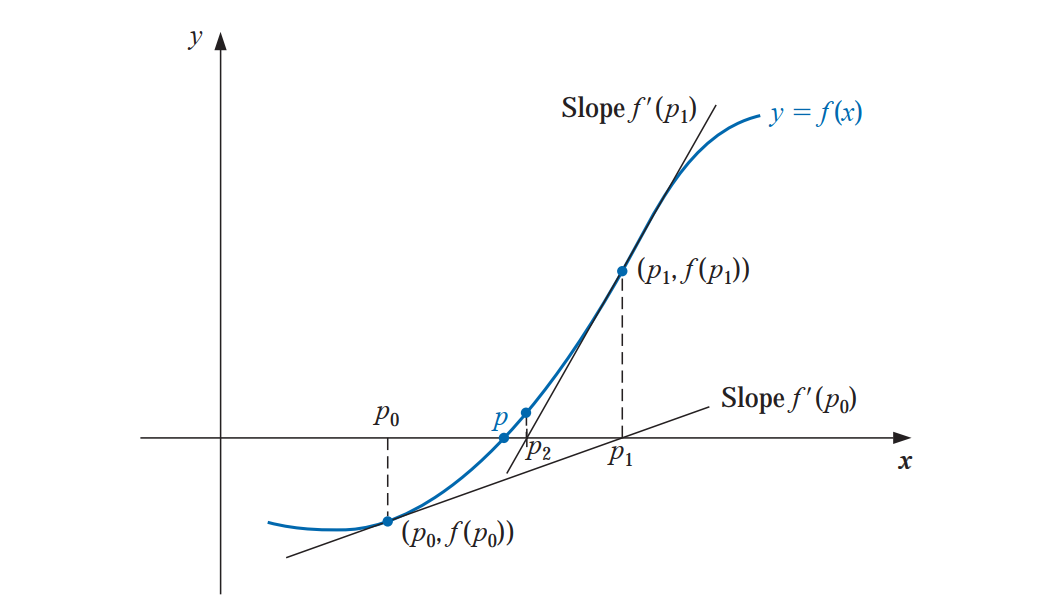
\includegraphics[width=1\linewidth]{figures/newton method.png}
    \caption{Minh họa hình học của phương pháp Newton}
    \label{fig:placeholder}
\end{figure}

Hình~\ref{fig:placeholder} minh họa cách các giá trị xấp xỉ được xác định thông qua các tiếp tuyến liên tiếp. 
Bắt đầu từ giá trị xấp xỉ ban đầu $p_0$, giá trị xấp xỉ kế tiếp $p_1$ được xác định là hoành độ của giao điểm giữa trục hoành và tiếp tuyến của đồ thị hàm $f$ tại điểm $(p_0, f(p_0))$. Tương tự, giá trị xấp xỉ $p_2$ là hoành độ của giao điểm giữa trục hoành và tiếp tuyến của đồ thị $f$ tại điểm $(p_1, f(p_1))$, và quá trình này tiếp tục như vậy. 

\subsubsection*{Thuật toán}

\begin{algorithm}[H]
\caption{Phương pháp Newton}
\label{alg:newton}
\begin{algorithm}[!h]
\SetAlgoLined
\KwIn{
    Hàm $f(x)$, đạo hàm $f'(x)$;\\
    Giá trị ban đầu $p_0$;\\
    Sai số cho phép $\mathrm{TOL}$;\\
    Số lần lặp tối đa $N_0$.
}
\KwOut{
    Nghiệm xấp xỉ $p$ hoặc thông báo lỗi nếu phương pháp thất bại.
}
\BlankLine
\caption{Thuật toán Newton–Raphson}
\label{alg:newton_method}
\end{algorithm}


\BlankLine
\textbf{Bước 1.} Đặt $i = 1$. \\
\textbf{Bước 2.} \While{$i \leq N_0$}{
    Tính $p = p_0 - \dfrac{f(p_0)}{f'(p_0)}$. \\
    \If{$|p - p_0| < \text{TOL}$}{
        Xuất $p$ (nghiệm xấp xỉ) và \textbf{dừng}.}
    Cập nhật $p_0 = p$. \\
    Tăng $i = i + 1$.
}
\textbf{Bước 3.} Nếu $i > N_0$, xuất thông báo: “Phương pháp thất bại sau $N_0$ lần lặp.”
\end{algorithm}

\subsubsection*{Điều kiện dừng}

Trong quá trình lặp của phương pháp Newton, ta cần xác định tiêu chí dừng thích hợp 
để kết luận rằng nghiệm xấp xỉ $p_n$ đã đủ gần với nghiệm thực $p$ của phương trình $f(x)=0$. 
Thông thường, một trong ba điều kiện sau được sử dụng:

\begin{enumerate}
    \item \textbf{Sai số tuyệt đối nhỏ:}
    \[
        |p_{n} - p_{n-1}| < \varepsilon,
    \]
    với $\varepsilon$ là sai số cho phép (tolerance). 
    Điều kiện này đảm bảo hai lần lặp liên tiếp cho kết quả gần nhau.

    \item \textbf{Sai số tương đối nhỏ:}
    \[
        \frac{|p_{n} - p_{n-1}|}{|p_{n}|} < \varepsilon.
    \]
    Điều kiện này thường được dùng khi giá trị nghiệm có thể lớn hoặc nhỏ, 
    giúp kiểm soát mức độ chính xác tương đối.

    \item \textbf{Giá trị hàm gần bằng 0:}
    \[
        |f(p_n)| < \varepsilon.
    \]
    Điều kiện này đảm bảo rằng $p_n$ gần với nghiệm thực của $f(x)=0$ về mặt giá trị hàm.
\end{enumerate}

\subsubsection*{Đặc điểm hội tụ của phương pháp Newton}

Giả sử $f \in C^2[a,b]$, $p$ là nghiệm thực của phương trình $f(x) = 0$, 
và $f'(p) \neq 0$. Khi đó, nếu giá trị khởi tạo $p_0$ được chọn đủ gần với $p$, 
dãy $\{p_n\}$ được xác định bởi công thức lặp
\[
    p_{n} = p_{n-1} - \frac{f(p_{n-1})}{f'(p_{n-1})},
\]
sẽ \textbf{hội tụ bậc hai} (quadratic convergence) về nghiệm $p$.

Điều này có nghĩa là tồn tại một hằng số $C > 0$ sao cho
\[
    |p_{n+1} - p| \leq C\,|p_n - p|^2.
\]
Nói cách khác, \emph{sai số của lần lặp tiếp theo tỉ lệ với bình phương sai số của lần lặp trước đó}. 
Do đó, khi dãy $\{p_n\}$ tiến gần nghiệm, số chữ số chính xác trong nghiệm xấp xỉ gần như tăng gấp đôi sau mỗi bước lặp.

\begin{center}
\textit{Tốc độ hội tụ bậc hai là ưu điểm nổi bật nhất của phương pháp Newton.}
\end{center}

Tuy nhiên, phương pháp này chỉ đảm bảo hội tụ nhanh khi các điều kiện sau được thỏa mãn:
\begin{enumerate}
    \item Hàm $f(x)$ khả vi liên tục và $f'(x)$ không triệt tiêu trong lân cận của nghiệm $p$.
    \item Giá trị ban đầu $p_0$ được chọn đủ gần nghiệm thực $p$.
    \item Đạo hàm $f'(x)$ có thể được tính chính xác hoặc xấp xỉ tốt.
\end{enumerate}

Nếu các điều kiện trên không được thỏa mãn, phương pháp Newton có thể:
\begin{itemize}
    \item hội tụ chậm hoặc phân kỳ (diverge),
    \item dao động giữa các giá trị (oscillate),
    \item hoặc hội tụ về một nghiệm khác không mong muốn.
\end{itemize}

\noindent
Ví dụ, nếu $f'(p_0) = 0$, công thức lặp sẽ không xác định do mẫu số bằng không. Vì vậy, trong thực hành tính toán, việc chọn giá trị ban đầu $p_0$ hợp lý và kiểm tra đạo hàm $f'(x)$ là bước rất quan trọng trước khi áp dụng phương pháp Newton.

\newtheorem{theorem}{Định lý}
\begin{theorem}
Giả sử $f \in C^2[a, b]$. 
Nếu tồn tại $p \in (a, b)$ sao cho $f(p) = 0$ và $f'(p) \neq 0$, 
thì tồn tại $\delta > 0$ sao cho phương pháp Newton sinh ra dãy 
$\{p_n\}_{n=1}^{\infty}$ hội tụ về $p$ với mọi giá trị khởi tạo 
$p_0 \in [p - \delta,\, p + \delta]$.
\end{theorem}

\subsubsection*{Ví dụ minh họa}

Xét phương trình
\[
    f(x) = \cos x - x = 0.
\]
Ta sẽ sử dụng phương pháp Newton để tìm nghiệm xấp xỉ của phương trình này.

\textbf{Bước 1. Xác định đạo hàm.}
\[
    f'(x) = -\sin x - 1.
\]

\textbf{Bước 2. Chọn giá trị khởi tạo.}
Chọn $p_0 = \frac{\pi}{4} \approx 0.785398$.

\textbf{Bước 3. Áp dụng công thức Newton.}
\[
    p_{n} = p_{n-1} - \frac{f(p_{n-1})}{f'(p_{n-1})} 
           = p_{n-1} - \frac{\cos(p_{n-1}) - p_{n-1}}{-\sin(p_{n-1}) - 1}.
\]

\textbf{Bước 4. Thực hiện các bước lặp.}
Ta thu được các giá trị sau:

\begin{center}
\begin{tabular}{|c|c|}
\hline
\textbf{Lần lặp} $n$ & \textbf{Giá trị xấp xỉ} $p_n$ \\
\hline
0 & 0.7853981635 \\
1 & 0.7395361337 \\
2 & 0.7390851781 \\
3 & 0.7390851332 \\
\hline
\end{tabular}
\end{center}

\textbf{Kết quả.}
Sau ba lần lặp, dãy $\{p_n\}$ hội tụ đến nghiệm
\[
    p \approx 0.7390851332,
\]
chính là nghiệm của phương trình $x = \cos x$.

\subsubsection*{Ví dụ minh họa}
\begin{itemize}
    \item Sai số giảm rất nhanh sau mỗi lần lặp, phản ánh tính \textbf{hội tụ bậc hai} của phương pháp Newton.
    \item Nếu chọn giá trị ban đầu $p_0$ nằm xa nghiệm thật, quá trình có thể phân kỳ hoặc dao động.
    \item Trong thực hành, có thể dừng khi $|p_{n} - p_{n-1}| < 10^{-6}$ hoặc $|f(p_n)| < 10^{-6}$.
\end{itemize}

\subsection{Các mở rộng của phương pháp Newton}
\subsubsection{Phương pháp Secant}
Phương pháp Secant là một mở rộng của phương pháp Newton, 
nhằm khắc phục nhược điểm cần tính đạo hàm $f'(x)$ tại mỗi bước lặp. 
Thay vì tính đạo hàm chính xác, phương pháp này sử dụng \textbf{sai phân hữu hạn} để xấp xỉ đạo hàm.

\paragraph*{Ý tưởng.}
Xuất phát từ công thức Newton:
\[
    p_{n} = p_{n-1} - \frac{f(p_{n-1})}{f'(p_{n-1})},
\]
thay đạo hàm $f'(p_{n-1})$ bằng sai phân:
\[
    f'(p_{n-1}) \approx 
    \frac{f(p_{n-1}) - f(p_{n-2})}{p_{n-1} - p_{n-2}}.
\]
Khi đó, công thức lặp trở thành:
\[
    p_{n} = p_{n-1} - f(p_{n-1})
    \frac{p_{n-1} - p_{n-2}}{f(p_{n-1}) - f(p_{n-2})}.
\]

\begin{figure}[H]
    \centering
    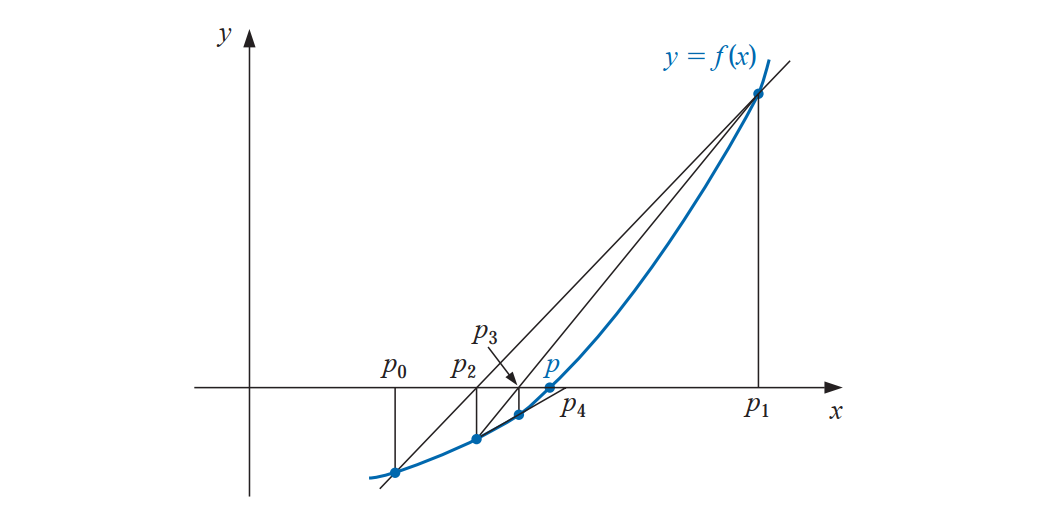
\includegraphics[width=1\linewidth]{figures/secant.png}
    \caption{Minh họa hình học của phương pháp Secant}
    \label{fig:placeholder}
\end{figure}

Bắt đầu với hai giá trị xấp xỉ ban đầu $p_0$ và $p_1$, 
giá trị xấp xỉ $p_2$ được xác định là \textbf{hoành độ của giao điểm giữa trục hoành và đường thẳng nối hai điểm} $(p_0, f(p_0))$ và $(p_1, f(p_1))$ trên đồ thị hàm $f$. Tương tự, giá trị xấp xỉ $p_3$ là hoành độ của giao điểm giữa trục hoành và đường thẳng nối hai điểm $(p_1, f(p_1))$ và $(p_2, f(p_2))$, và quá trình này tiếp tục như vậy.
Lưu ý rằng kể từ khi $p_2$ được xác định, mỗi bước của phương pháp Secant \textbf{chỉ cần một lần tính giá trị hàm $f(x)$}. 
Ngược lại, mỗi bước của phương pháp Newton yêu cầu đánh giá cả 
\textbf{hàm $f(x)$ và đạo hàm $f'(x)$}.

\paragraph*{Thuật toán Secant.}
\begin{enumerate}
    \item Chọn hai giá trị khởi tạo $p_0$ và $p_1$, cùng sai số cho phép $\text{TOL}$ và số lần lặp tối đa $N_0$.
    \item Với $i = 2, 3, \ldots, N_0$:
    \begin{enumerate}
        \item Tính
        \[
            p_i = p_{i-1} - f(p_{i-1})
            \frac{p_{i-1} - p_{i-2}}{f(p_{i-1}) - f(p_{i-2})}.
        \]
        \item Nếu $|p_i - p_{i-1}| < \text{TOL}$ hoặc $|f(p_i)| < \text{TOL}$, dừng và xuất $p_i$.
        \item Ngược lại, gán $p_{i-2} = p_{i-1}$ và $p_{i-1} = p_i$ rồi tiếp tục.
    \end{enumerate}
    \item Nếu vượt quá $N_0$ lần lặp, thông báo “Phương pháp thất bại”.
\end{enumerate}

\paragraph*{Đặc điểm.}
\begin{itemize}
    \item Không cần tính đạo hàm $f'(x)$.
    \item Cần hai giá trị khởi tạo $p_0$ và $p_1$.
    \item Tốc độ hội tụ \textbf{siêu tuyến tính} với bậc khoảng $1.618$ (bằng số vàng).
    \item Có thể phân kỳ nếu $p_0$ và $p_1$ không đủ gần nghiệm thật.
\end{itemize}

\paragraph*{Ví dụ minh họa.}
Giải phương trình $f(x) = \cos x - x = 0$ bằng phương pháp Secant 
với $p_0 = 0.5$, $p_1 = 0.785398$.

\begin{center}
\begin{tabular}{|c|c|}
\hline
\textbf{Lần lặp} $n$ & \textbf{Giá trị xấp xỉ} $p_n$ \\
\hline
0 & 0.5000000000 \\
1 & 0.7853980000 \\
2 & 0.7362990000 \\
3 & 0.7391190000 \\
4 & 0.7390851000 \\
\hline
\end{tabular}
\end{center}

Sau vài lần lặp, ta được $p \approx 0.7390851$, 
rất gần với nghiệm thật của phương trình $x = \cos x$.

\paragraph*{Nhận xét.}
Phương pháp Secant thường được ưa dùng khi:
\begin{itemize}
    \item đạo hàm của $f(x)$ khó hoặc tốn kém để tính toán;
    \item hoặc ta chỉ có giá trị hàm tại các điểm đã biết.
\end{itemize}
Tuy tốc độ hội tụ của phương pháp Secant chậm hơn Newton (bậc $\approx 1.618 < 2$), nhưng ưu điểm là \textbf{không cần đạo hàm}, giúp nó linh hoạt và hiệu quả hơn trong nhiều bài toán thực tế.

\subsubsection*{Phương pháp False Position}

Phương pháp \textit{False Position} hay còn gọi là \textit{Regula Falsi} 
là một biến thể của phương pháp Secant. 
Tương tự Secant, nó dùng đường thẳng đi qua hai điểm trên đồ thị hàm $f(x)$ 
để xấp xỉ nghiệm của phương trình $f(x) = 0$, 
nhưng có điểm khác biệt quan trọng là \textbf{đảm bảo nghiệm luôn nằm trong đoạn ban đầu}.

\paragraph*{Ý tưởng.}
Giả sử ta có hai điểm ban đầu $a$ và $b$ sao cho
\[
    f(a) \cdot f(b) < 0,
\]
tức là $f(x)$ đổi dấu trên đoạn $[a, b]$ và do đó tồn tại ít nhất một nghiệm $p \in (a, b)$ 
theo định lý giá trị trung gian.  
Phương pháp False Position xác định nghiệm xấp xỉ đầu tiên bằng công thức Secant:
\[
    p = b - f(b)\frac{b - a}{f(b) - f(a)}.
\]
Nếu $f(a)f(p) < 0$, ta thay $b = p$; ngược lại, nếu $f(b)f(p) < 0$, ta thay $a = p$.  
Quá trình được lặp lại cho đến khi đạt sai số mong muốn.

\begin{figure}[H]
    \centering
    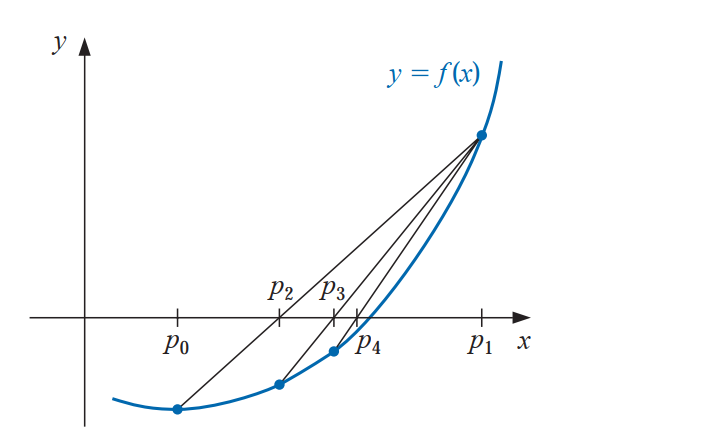
\includegraphics[width=1\linewidth]{figures/fasle position.png}
    \caption{Minh họa hình học của phương pháp False Position}
    \label{fig:placeholder}
\end{figure}


\paragraph*{Thuật toán False Position.}
\begin{enumerate}
    \item Cho hai giá trị $a$ và $b$ sao cho $f(a)f(b) < 0$.
    \item Tính $p$ bằng:
    \[
        p = b - f(b)\frac{b - a}{f(b) - f(a)}.
    \]
    \item Nếu $|f(p)| < \text{TOL}$ hoặc $|b - a| < \text{TOL}$, dừng và xuất $p$.
    \item Nếu $f(a)f(p) < 0$, gán $b = p$; ngược lại, gán $a = p$.
    \item Lặp lại các bước trên cho đến khi đạt điều kiện dừng.
\end{enumerate}

\paragraph*{Đặc điểm.}
\begin{itemize}
    \item Phương pháp False Position luôn \textbf{duy trì đoạn chứa nghiệm}, 
    nên đảm bảo hội tụ (giống phương pháp chia đôi).
    \item Tuy nhiên, tốc độ hội tụ chỉ là \textbf{tuyến tính}, 
    chậm hơn phương pháp Newton và Secant.
    \item Nếu $f(x)$ có độ dốc lớn ở một đầu đoạn, các giá trị $a$ hoặc $b$ có thể bị “cố định”, 
    làm quá trình hội tụ rất chậm.
\end{itemize}

\paragraph*{Ví dụ minh họa.}
Giải phương trình $f(x) = \cos x - x = 0$ bằng phương pháp False Position 
với đoạn ban đầu $[a, b] = [0, 1]$.

\begin{center}
\begin{tabular}{|c|c|c|c|}
\hline
\textbf{Lần lặp} $n$ & $a_n$ & $b_n$ & $p_n$ \\
\hline
0 & 0.000000 & 1.000000 & 0.685074 \\
1 & 0.685074 & 1.000000 & 0.736299 \\
2 & 0.736299 & 1.000000 & 0.739119 \\
3 & 0.739119 & 1.000000 & 0.739085 \\
\hline
\end{tabular}
\end{center}

Kết quả thu được sau vài bước lặp là 
\[
    p \approx 0.739085,
\]
trùng với nghiệm thật của phương trình $x = \cos x$.

\paragraph*{Nhận xét.}
\begin{itemize}
    \item Phương pháp False Position kết hợp ưu điểm của phương pháp chia đôi (đảm bảo hội tụ) và phương pháp Secant (hội tụ nhanh hơn).
    \item Dù vậy, trong thực tế, nếu cần hội tụ nhanh hơn, người ta thường dùng \textbf{phương pháp Secant} hoặc \textbf{Newton}.
\end{itemize}

\section{Phân tích sai số trong các phương pháp lặp}

\subsection{Bậc hội tụ (Order of Convergence)}
\subsubsection*{Định nghĩa bậc hội tụ}

Giả sử $\{p_n\}$ là dãy các giá trị xấp xỉ hội tụ đến nghiệm thực $p$ của một phương trình $f(x) = 0$, và đặt sai số tại bước $n$ là 
\[
e_n = p_n - p.
\]
Dãy $\{p_n\}$ được gọi là \textbf{hội tụ đến $p$ với bậc hội tụ $\alpha > 0$} nếu tồn tại một hằng số $\lambda \ge 0$ sao cho
\[
    \lim_{n \to \infty} 
    \frac{|p_{n+1} - p|}{|p_n - p|^{\alpha}} = \lambda.
\]

Khi đó:
\begin{itemize}
    \item $\alpha$ được gọi là \textbf{bậc hội tụ (order of convergence)};
    \item $\lambda$ được gọi là \textbf{hằng số hội tụ (rate constant)}.
\end{itemize}

\paragraph*{Các trường hợp đặc biệt:}
\begin{enumerate}
    \item Nếu $\alpha = 1$ và $0 < \lambda < 1$, dãy có \textbf{hội tụ tuyến tính}:
    \[
        |e_{n+1}| \approx \lambda |e_n|
    \]
    \item Nếu $\alpha = 2$, dãy có \textbf{hội tụ bậc hai}:
    \[
        |e_{n+1}| \approx \lambda |e_n|^2
    \]

\end{enumerate}

\paragraph*{Nhận xét:}
\begin{itemize}
    \item Bậc hội tụ càng cao thì phương pháp càng nhanh đạt đến nghiệm thật.
    \item Tuy nhiên, phương pháp có bậc hội tụ cao thường yêu cầu nhiều phép tính hơn mỗi bước 

\end{itemize}

\begin{theorem}
Giả sử $g \in C[a, b]$ và thỏa mãn $g(x) \in [a, b]$ với mọi $x \in [a, b]$. 
Giả sử thêm rằng $g$ khả vi trên $(a, b)$ và tồn tại một hằng số dương $k < 1$ sao cho
\[
    |g'(x)| \le k, \quad \forall x \in (a, b).
\]
Nếu $g'(p) \ne 0$, thì với mọi giá trị khởi tạo $p_0 \ne p$ trong $[a, b]$, 
dãy $\{p_n\}$ được xác định bởi
\[
    p_n = g(p_{n-1}), \quad n \ge 1,
\]
hội tụ \textbf{tuyến tính} đến \textbf{điểm cố định duy nhất} $p \in [a, b]$.
\end{theorem}

Trường hợp đặc biệt khi $g'(p) = 0$ dẫn đến tốc độ hội tụ nhanh hơn. 
Kết quả sau đây chỉ ra rằng khi đó, dãy lặp sẽ hội tụ ít nhất với bậc hai.

\begin{theorem}
Giả sử $p$ là nghiệm của phương trình $x = g(x)$. 
Giả sử thêm rằng $g'(p) = 0$ và $g$ khả vi liên tục trên một khoảng mở $I$ chứa $p$, với $|g''(x)| < M$ trên $I$ cho một hằng số dương $M$.

Khi đó tồn tại $\delta > 0$ sao cho với mọi giá trị khởi tạo 
$p_0 \in [p - \delta,\, p + \delta]$, dãy lặp
\[
    p_n = g(p_{n-1}), \quad n \ge 1,
\]
hội tụ \textbf{ít nhất bậc hai} đến $p$. Hơn nữa, với $n$ đủ lớn, ta có ước lượng sai số:
\[
    |p_{n+1} - p| < \frac{M}{2}\, |p_n - p|^2.
\]
\end{theorem}

\paragraph*{Hàm lặp và điều kiện hội tụ bậc hai}
Hai định lý trên cho thấy rằng, để một phương pháp lặp dạng cố định đạt được tốc độ hội tụ bậc hai, 
ta cần xây dựng hàm lặp $g(x)$ sao cho:
\[
    g(p) = p \quad \text{và} \quad g'(p) = 0.
\]
Một cách tự nhiên để xây dựng hàm như vậy từ phương trình $f(x) = 0$
là cộng hoặc trừ một bội số của $f(x)$ vào $x$. 
Xét dãy lặp dạng
\[
    p_n = g(p_{n-1}), \quad n \ge 1,
\]
với
\[
    g(x) = x - \phi(x) f(x),
\]
trong đó $\phi(x)$ là một hàm khả vi sẽ được xác định sao cho quá trình lặp hội tụ nhanh.
Tính đạo hàm của $g(x)$:
\[
    g'(x) = 1 - \phi'(x)f(x) - \phi(x)f'(x).
\]
Tại nghiệm $p$ của $f(x) = 0$, ta có $f(p) = 0$, nên:
\[
    g'(p) = 1 - \phi(p)f'(p).
\]
Để đạt được hội tụ bậc hai, ta cần $g'(p) = 0$, do đó:
\[
    \phi(p) = \frac{1}{f'(p)}.
\]
Nếu ta chọn $\phi(x) = 1 / f'(x)$, thì điều kiện trên được thỏa mãn, và phương pháp lặp thu được chính là:
\[
    p_n = p_{n-1} - \frac{f(p_{n-1})}{f'(p_{n-1})},
\]
tức là \textbf{phương pháp Newton (Newton's Method)}.\\

Từ đó suy ra rằng, nếu $f(p) = 0$ và $f'(p) \ne 0$, 
thì với điểm khởi tạo $p_0$ đủ gần nghiệm thật $p$, 
phương pháp Newton hội tụ ít nhất với \textbf{bậc hai}. 
Điều này giải thích vì sao Newton’s Method 
là một trong những phương pháp tìm nghiệm nhanh và hiệu quả nhất trong thực hành.

\captionsetup[table]{skip=10pt}
\begin{table}[H]
\centering
\caption{\textit{Bảng so sánh bậc hội tụ của các phương pháp lặp phổ biến}}
\label{tab:order_of_convergence}
\begin{adjustbox}{max width=\textwidth}
\renewcommand{\arraystretch}{1.3} % add vertical spacing
\begin{tabularx}{\textwidth}{|l|>{\centering\arraybackslash}X|c|X|}
\hline
\textbf{Phương pháp} &
\textbf{Công thức lặp} &
\textbf{Bậc hội tụ $\alpha$} &
\textbf{Đặc điểm nổi bật} \\ \hline

Bisection &
$p_{n} = \dfrac{a_n + b_n}{2}$ &
$1.0$ (tuyến tính) &
Luôn hội tụ, nhưng chậm. \\ \hline

Fixed-Point &
$p_n = g(p_{n-1})$ &
$1.0$ &
Dễ cài đặt, phụ thuộc vào $|g'(p)| < 1$. \\ \hline

Secant &
$p_n = p_{n-1} - f(p_{n-1}) 
\dfrac{p_{n-1} - p_{n-2}}{f(p_{n-1}) - f(p_{n-2})}$ &
$\approx 1.618$ &
Không cần đạo hàm, hội tụ nhanh. \\ \hline

Newton &
$p_n = p_{n-1} - \dfrac{f(p_{n-1})}{f'(p_{n-1})}$ &
$2.0$ &
Rất nhanh, cần đạo hàm. \\ \hline

Modified Newton &
$p_n = p_{n-1} -
\dfrac{f(p_{n-1}) f'(p_{n-1})}
{[f'(p_{n-1})]^2 - f(p_{n-1}) f''(p_{n-1})}$ &
$3.0$ &
Cần đạo hàm bậc hai, hội tụ cực nhanh. \\ \hline
\end{tabularx}
\end{adjustbox}
\end{table}

\paragraph*{Kết luận.}
Bậc hội tụ là thước đo tốc độ tiệm cận nghiệm của các phương pháp lặp. 
Nó cho biết mức độ giảm sai số qua từng bước tính toán.

\subsection{Nghiệm bội (Multiple Roots)}

\paragraph*{Định nghĩa.}
Giả sử $f(x)$ là một hàm khả vi nhiều lần trên khoảng $I$, và $p$ là nghiệm của phương trình $f(x) = 0$. 
Khi đó, $p$ được gọi là \textbf{nghiệm bội $m$} (root of multiplicity $m$) của $f$ 
nếu:
\[
    f(p) = 0, \quad f'(p) = 0, \quad f''(p) = 0, \quad \dots, \quad f^{(m-1)}(p) = 0,
\]
nhưng
\[
    f^{(m)}(p) \ne 0.
\]
Nói cách khác, $p$ là nghiệm của $f(x)$ và đồng thời là nghiệm của tất cả các đạo hàm bậc nhỏ hơn $m$, nhưng không phải là nghiệm của đạo hàm bậc $m$.

\paragraph*{Ví dụ.}
\begin{itemize}
    \item Hàm $f(x) = (x - 2)^2$ có nghiệm bội $m = 2$ tại $p = 2$.
    \item Hàm $f(x) = (x - 1)^3$ có nghiệm bội $m = 3$ tại $p = 1$.
\end{itemize}

\paragraph*{Giải thích hình học.}
Nếu $p$ là nghiệm bội lớn hơn $1$, đồ thị của $f(x)$ 
\textbf{chạm} trục hoành tại $x = p$ nhưng không cắt qua nó.  
Ví dụ, với $f(x) = (x - 2)^2$, 
đồ thị tiếp xúc với trục hoành tại $x=2$ thay vì cắt qua, do đó Newton’s Method sẽ hội tụ chậm hơn trong vùng lân cận điểm này.
\\
Để mô tả rõ hơn hành vi này, các định lý sau đây trình bày chi tiết tốc độ hội tụ của phương pháp Newton cổ điển, phương pháp Newton cải tiến cho nghiệm bội, và phương pháp Secant.

% --- THEOREM 2.10 ---
\begin{theorem}
Giả sử $f \in C^{2}[a,b]$ và $p \in (a,b)$ là nghiệm bội $m$ của $f$, tức là
\[
    f(p) = f'(p) = \dots = f^{(m-1)}(p) = 0, \quad f^{(m)}(p) \ne 0.
\]
Nếu $p_0$ đủ gần $p$, thì dãy được xác định bởi công thức Newton
\[
    p_{n+1} = p_n - \frac{f(p_n)}{f'(p_n)}, \quad n \ge 0,
\]
hội tụ đến $p$ với \textbf{tốc độ tuyến tính} và hằng số hội tụ xấp xỉ
\[
    |p_{n+1} - p| \approx \frac{m-1}{m}\,|p_n - p|.
\]
\end{theorem}

\begin{theorem}
Giả sử $f \in C^{2}[a,b]$ và $p \in (a,b)$ là nghiệm bội $m$ của $f$. 
Khi đó, phương pháp Newton cải tiến
\[
    p_{n+1} = p_n - \frac{m\, f(p_n)}{f'(p_n)}, \quad n \ge 0,
\]
hội tụ đến $p$ với \textbf{bậc hội tụ hai} đối với mọi giá trị khởi tạo $p_0$ đủ gần $p$.
\end{theorem}

\begin{theorem}
Giả sử $f \in C^{2}[a,b]$ và $p$ là nghiệm đơn của $f$. 
Khi đó, phương pháp Secant 
\[
    p_{n} = p_{n-1} - f(p_{n-1}) \cdot 
    \frac{p_{n-1} - p_{n-2}}{f(p_{n-1}) - f(p_{n-2})}, \quad n \ge 2,
\]
hội tụ đến $p$ với \textbf{bậc hội tụ} xấp xỉ $\alpha \approx 1.618$, 
tức là tốc độ hội tụ \textbf{siêu tuyến tính (superlinear)}.
\end{theorem}

\paragraph*{Nhận xét:}
\begin{itemize}
    \item \textbf{Định lý~4} cho thấy khi nghiệm có bội số $m > 1$, 
    phương pháp Newton tiêu chuẩn chỉ hội tụ tuyến tính với hằng số hội tụ $\tfrac{m-1}{m}$.  
    Điều này giải thích hiện tượng hội tụ chậm khi đồ thị của $f(x)$ 
    tiếp xúc với trục hoành tại nghiệm (thay vì cắt qua).

    \item \textbf{Định lý~5} khắc phục hạn chế này bằng cách 
    nhân thêm hệ số $m$ trong công thức Newton.  
    Hệ số này hiệu chỉnh lại độ dốc tiếp tuyến và 
    khôi phục \textbf{tốc độ hội tụ bậc hai} như trong trường hợp nghiệm đơn.

    \item \textbf{Định lý~6} mô tả một phương pháp thay thế – 
    \textbf{phương pháp Secant} – 
    không yêu cầu đạo hàm, nhưng vẫn đạt tốc độ hội tụ nhanh 
    (bậc $\alpha \approx 1.618$).  
    Do đó, nó được xem là một sự cân bằng tốt giữa hiệu năng và chi phí tính toán.
\end{itemize}

\paragraph*{}
Ba định lý trên nhấn mạnh rằng:
\begin{itemize}
    \item Phương pháp Newton tiêu chuẩn có thể mất hiệu quả khi gặp nghiệm bội.
    \item Có thể khôi phục lại tốc độ hội tụ bậc hai 
    bằng cách sử dụng \textbf{phương pháp Newton cải tiến}.
    \item Trong các trường hợp không thể hoặc không muốn tính đạo hàm, 
    \textbf{phương pháp Secant} là lựa chọn hợp lý với tốc độ hội tụ siêu tuyến tính.
\end{itemize}
\subsubsection*{Ví dụ: Ảnh hưởng của nghiệm bội đến tốc độ hội tụ của Newton}

\paragraph*{}
Xét hàm
\[
    f(x) = e^x - x - 1.
\]
\begin{enumerate}
    \item Chứng minh rằng $f$ có nghiệm bội $2$ tại $x = 0$.
    \item Chứng minh rằng phương pháp Newton với $p_0 = 1$ hội tụ đến nghiệm này, 
    nhưng không hội tụ bậc hai.
\end{enumerate}

\paragraph*{(1) Chứng minh $x = 0$ là nghiệm bội $2$.}
Ta có
\[
    f(x) = e^x - x - 1, \quad f'(x) = e^x - 1, \quad f''(x) = e^x.
\]
Khi $x = 0$, ta được:
\[
    f(0) = 1 - 0 - 1 = 0, \quad f'(0) = 1 - 1 = 0, \quad f''(0) = 1 \ne 0.
\]
Do đó, $x = 0$ là \textbf{nghiệm bội $2$} của phương trình $f(x) = 0$.

\paragraph*{(2) Phân tích hội tụ của phương pháp Newton.}
Phương pháp Newton có công thức lặp:
\[
    p_{n+1} = p_n - \frac{f(p_n)}{f'(p_n)}.
\]
Thay $f(x) = e^x - x - 1$ và $f'(x) = e^x - 1$ vào ta được:
\[
    p_{n+1} = p_n - \frac{e^{p_n} - p_n - 1}{e^{p_n} - 1}.
\]

\paragraph*{Tính gần nghiệm $x = 0$.}
Khai triển $e^x$ quanh $x=0$:
\[
    e^x = 1 + x + \frac{x^2}{2} + O(x^3).
\]
Khi đó:
\[
    f(x) = \frac{x^2}{2} + O(x^3), \quad f'(x) = x + \frac{x^2}{2} + O(x^3).
\]
Suy ra:
\[
    \frac{f(x)}{f'(x)} 
    = \frac{\tfrac{x^2}{2} + O(x^3)}{x + \tfrac{x^2}{2} + O(x^3)} 
    = \frac{x}{2} + O(x^2).
\]
Do đó, phép lặp Newton gần nghiệm có dạng:
\[
    p_{n+1} = p_n - \frac{f(p_n)}{f'(p_n)} = p_n - \left( \frac{p_n}{2} + O(p_n^2) \right)
    = \frac{p_n}{2} + O(p_n^2).
\]
Bỏ qua thành phần bậc cao, ta có xấp xỉ:
\[
    |p_{n+1}| \approx \frac{1}{2} |p_n|.
\]

\paragraph*{Kết luận}
Sai số giảm xấp xỉ một nửa sau mỗi lần lặp, nghĩa là phương pháp Newton 
\textbf{hội tụ tuyến tính} với hằng số hội tụ $\lambda = \tfrac{1}{2}$, thay vì hội tụ bậc hai như trong trường hợp nghiệm đơn.

Nếu chọn $p_0 = 1$, ta có:
\[
\begin{array}{c|c}
n & p_n \\ \hline
0 & 1.000000 \\
1 & 0.53788284 \\
2 & 0.25577441 \\
3 & 0.12604745 \\
4 & 0.06285013 \\
5 & 0.03133119 \\
\end{array}
\]
Ta nhận thấy rằng $p_n \to 0$, nhưng giá trị giảm gần \emph{một nửa} sau mỗi bước, 
khớp với tốc độ hội tụ tuyến tính dự đoán ở trên.

\paragraph*{Nhận xét.}
Ví dụ này minh họa rằng:
\begin{itemize}
    \item Khi nghiệm là nghiệm bội, phương pháp Newton thông thường không còn hội tụ bậc hai.
    \item Trong trường hợp này ($m = 2$), tốc độ hội tụ chỉ còn tuyến tính với hệ số $\tfrac{1}{2}$.
    \item Nếu áp dụng \textbf{phương pháp Newton cải tiến}:
    \[
        p_{n+1} = p_n - \frac{2 f(p_n)}{f'(p_n)},
    \]
    thì hội tụ sẽ trở lại bậc hai như với nghiệm đơn.
\end{itemize}

\paragraph*{Nhận xét.}
\begin{itemize}
    \item Sai số giảm rất nhanh sau mỗi vòng lặp, 
    chứng tỏ phương pháp Newton có hiệu quả vượt trội 
    khi giá trị khởi tạo đủ gần nghiệm thật.
    \item Bậc hội tụ thực nghiệm $\alpha \approx 2$ khớp với 
    kết quả lý thuyết trong phần “Order of Convergence”.
    \item Nếu nghiệm là nghiệm bội, tốc độ hội tụ sẽ giảm 
    xuống tuyến tính như đã nêu trong Định lý~4.
\end{itemize}

\section{Tăng tốc hội tụ (Accelerating Convergence)}

Trong các phần trước, ta đã xem xét các phương pháp lặp 
và phân tích tốc độ hội tụ của chúng thông qua khái niệm \textit{bậc hội tụ}.
Ta đã thấy rằng các phương pháp như Newton’s Method có thể đạt \textbf{bậc hội tụ hai},
trong khi nhiều phương pháp khác – chẳng hạn như \textit{phương pháp cố định điểm} 
hoặc \textit{phương pháp dây cung} – chỉ đạt được \textbf{hội tụ tuyến tính} hoặc 
\textbf{siêu tuyến tính}.

Mặc dù các phương pháp hội tụ tuyến tính có ưu điểm là dễ tính toán,
nhưng chúng thường cần rất nhiều bước lặp để đạt được độ chính xác mong muốn.
Điều này làm tăng đáng kể chi phí tính toán khi áp dụng trong thực tế.
Vì vậy, một hướng tiếp cận tự nhiên là tìm cách \textbf{tăng tốc quá trình hội tụ}
mà không phải thay đổi bản chất của phương pháp lặp ban đầu.
Phần này giới thiệu hai kỹ thuật phổ biến được sử dụng cho mục đích đó:
\textbf{Aitken’s $\Delta^2$ Process} và \textbf{Steffensen’s Method}.
Hai phương pháp này có thể biến một dãy hội tụ tuyến tính thành một dãy hội tụ nhanh hơn, thậm chí đạt tới bậc hai trong nhiều trường hợp.

\subsection{Aitken’s $\Delta^2$ Process}

\paragraph*{Ý tưởng.}
Giả sử $\{p_n\}$ là một dãy hội tụ tuyến tính đến $p$, tức là tồn tại hằng số $0 < \lambda < 1$ sao cho
\[
    p_{n+1} - p \approx \lambda (p_n - p).
\]
Trong trường hợp như vậy, hội tụ thường diễn ra khá chậm.  
Mục tiêu của \textbf{phép biến đổi Aitken’s $\Delta^2$} 
là tạo ra một dãy mới $\{\hat{p}_n\}$ hội tụ nhanh hơn đến cùng giới hạn $p$.

\paragraph*{Công thức biến đổi.}
Gọi sai phân bậc nhất và bậc hai của dãy $\{p_n\}$ lần lượt là:
\[
    \Delta p_n = p_{n+1} - p_n, \qquad
    \Delta^2 p_n = \Delta p_{n+1} - \Delta p_n = p_{n+2} - 2p_{n+1} + p_n.
\]
Phép biến đổi Aitken định nghĩa dãy mới:
\[
    \hat{p}_n = p_n - \frac{(\Delta p_n)^2}{\Delta^2 p_n}
    = p_n - \frac{(p_{n+1} - p_n)^2}{p_{n+2} - 2p_{n+1} + p_n}.
\]
Nếu $\{p_n\}$ hội tụ tuyến tính, thì $\{\hat{p}_n\}$ thường hội tụ nhanh hơn đáng kể, 
thậm chí \textbf{siêu tuyến tính} trong nhiều trường hợp.

\paragraph*{Giải thích trực giác.}
Phép biến đổi này dựa trên việc \emph{nội suy tuyến tính} 
ba giá trị liên tiếp $p_n, p_{n+1}, p_{n+2}$ 
để ước lượng trực tiếp giới hạn $p$.  
Thay vì chờ dãy $\{p_n\}$ dần tiến tới $p$, 
Aitken’s process sử dụng dạng sai phân để dự đoán trước điểm hội tụ.

\paragraph*{Ví dụ minh họa.}
Xét dãy hội tụ tuyến tính:
\[
    p_n = 1 + \frac{1}{2^n}, \quad n = 0,1,2,\dots
\]
Rõ ràng $p = 1$.  
Ta tính:
\[
    p_0 = 1.5, \quad p_1 = 1.25, \quad p_2 = 1.125.
\]
Khi đó:
\[
    \Delta p_0 = p_1 - p_0 = -0.25, \quad
    \Delta^2 p_0 = p_2 - 2p_1 + p_0 = 0.125.
\]
Áp dụng công thức Aitken:
\[
    \hat{p}_0 = p_0 - \frac{(\Delta p_0)^2}{\Delta^2 p_0}
               = 1.5 - \frac{(-0.25)^2}{0.125} = 1.5 - 0.5 = 1.0.
\]
Chỉ sau một bước, ta đã thu được chính xác nghiệm $p = 1$, 
trong khi dãy gốc cần vô hạn bước để đạt tới giới hạn đó.  
Điều này cho thấy sức mạnh của Aitken’s $\Delta^2$ process 
trong việc tăng tốc hội tụ.

\paragraph*{Lưu ý.}
\begin{itemize}
    \item Phép biến đổi Aitken chỉ áp dụng hiệu quả khi dãy $\{p_n\}$ 
    hội tụ tuyến tính và $\Delta^2 p_n \ne 0$.
    \item Nếu dãy gốc đã hội tụ siêu tuyến tính hoặc bậc hai, 
    việc áp dụng Aitken có thể không cải thiện đáng kể (hoặc làm nhiễu kết quả do sai số làm tròn).
\end{itemize}

\paragraph*{Kết luận.}
Phương pháp Aitken’s $\Delta^2$ là một công cụ đơn giản nhưng hiệu quả 
để cải thiện tốc độ hội tụ của các dãy tuyến tính.  

\subsection{Steffensen’s Method}

\paragraph*{Ý tưởng.}
Phương pháp của Steffensen được xây dựng bằng cách 
áp dụng \textbf{Aitken’s $\Delta^2$ Process} trực tiếp cho 
\textit{phương pháp lặp cố định điểm}:
\[
    p_{n+1} = g(p_n).
\]
Mục tiêu là cải thiện tốc độ hội tụ của quá trình lặp này, 
đặc biệt khi nó chỉ hội tụ tuyến tính.

\paragraph*{Cơ sở lý thuyết.}
Nếu ta gọi:
\[
    p_{n+1} = g(p_n), \qquad 
    p_{n+2} = g(p_{n+1}),
\]
thì theo công thức của Aitken, 
giá trị được tăng tốc bởi Steffensen là:
\[
    \hat{p}_n = p_n - 
    \frac{(p_{n+1} - p_n)^2}{p_{n+2} - 2p_{n+1} + p_n}.
\]
Thay $p_{n+1} = g(p_n)$ và $p_{n+2} = g(g(p_n))$, 
ta thu được công thức của \textbf{Steffensen’s Method}:
\[
    p_{n+1} = p_n - 
    \frac{[g(p_n) - p_n]^2}{g(g(p_n)) - 2g(p_n) + p_n}.
\]
Phương pháp này không yêu cầu đạo hàm của $f(x)$, 
nhưng trong nhiều trường hợp vẫn đạt tốc độ hội tụ bậc hai.

\paragraph*{Liên hệ với Newton’s Method.}
Nếu ta chọn
\[
    g(x) = x - \frac{f(x)}{f'(x)},
\]
thì Steffensen’s Method trở thành Newton’s Method.  
Do đó, Steffensen có thể xem là một cách 
\textbf{ước lượng đạo hàm} trong Newton bằng sai phân hữu hạn.

\paragraph*{Ví dụ minh họa.}
Xét phương trình
\[
    f(x) = e^{-x} - x = 0,
\]
với phương pháp lặp cố định điểm
\[
    g(x) = e^{-x}.
\]
Chọn giá trị khởi tạo $p_0 = 0$, ta có:
\[
\begin{aligned}
    g(p_0) &= e^{0} = 1, \\
    g(g(p_0)) &= e^{-1} \approx 0.3679.
\end{aligned}
\]
Áp dụng công thức Steffensen:
\[
    p_1 = p_0 - 
    \frac{[g(p_0) - p_0]^2}{g(g(p_0)) - 2g(p_0) + p_0}
        = 0 - \frac{(1 - 0)^2}{0.3679 - 2(1) + 0}
        \approx 0.6127.
\]
Tiếp tục lặp thêm vài bước, ta thu được:
\[
\begin{array}{c|c}
n & p_n \\ \hline
0 & 0.0000 \\
1 & 0.6127 \\
2 & 0.5666 \\
3 & 0.5671 \\
\end{array}
\]
Nghiệm đúng là $p = 0.567143$, 
và chỉ sau vài vòng lặp, phương pháp đã hội tụ rất nhanh 
mà không cần đạo hàm của $f$.

\paragraph*{Đặc điểm.}
\begin{itemize}
    \item Không yêu cầu đạo hàm $f'(x)$, chỉ cần giá trị của hàm $g(x)$.
    \item Hội tụ bậc hai nếu $g'(p) \ne 1$.
    \item Thích hợp cho các bài toán mà việc tính đạo hàm là phức tạp hoặc tốn kém.
\end{itemize}

\paragraph*{Kết luận.}
Phương pháp của Steffensen là một trong những kỹ thuật 
\textbf{tăng tốc hội tụ} quan trọng nhất trong giải tích số.
Nó kết hợp sự đơn giản của phương pháp lặp cố định điểm với tốc độ hội tụ của phương pháp Newton, mà không cần sử dụng đạo hàm.
\section{Tìm nghiệm của đa thức và phương pháp 
(MüllerZeros of Polynomials and Müller's Method)}

\subsection{Đa thức đại số (Algebraic Polynomials)}

Một đa thức đại số bậc $n$ được viết dưới dạng tổng quát:
\[
P(x) = a_nx^n + a_{n-1}x^{n-1} + \cdots + a_1x + a_0,
\]
trong đó $a_i$ là các hệ số thực hoặc phức, và $a_n \neq 0$.

Theo \textit{Định lý cơ bản của Đại số} (\textit{Fundamental Theorem of Algebra}), mỗi đa thức bậc $n$ có đúng $n$ nghiệm phức (tính cả bội).  
Nếu tất cả hệ số $a_i$ là số thực, thì các nghiệm phức xuất hiện theo cặp liên hợp phức.

Mục tiêu là tìm các nghiệm $r$ sao cho $P(r) = 0$. Trong thực tế, các nghiệm này thường được tìm gần đúng bằng các phương pháp số, vì nghiệm chính xác chỉ biểu diễn được tường minh khi đa thức có bậc nhỏ hơn hoặc bằng 4.

\subsection{Phương pháp Horner (Horner’s Method)}

Phương pháp Horner là một kỹ thuật hiệu quả để \textit{tính giá trị của đa thức} và thực hiện \textit{chia đa thức} cho $(x - x_0)$.  
Nó giúp giảm đáng kể số phép nhân và cộng cần thiết, đồng thời tăng độ ổn định số.

Cho đa thức:
\[
P(x) = a_nx^n + a_{n-1}x^{n-1} + \cdots + a_1x + a_0.
\]
Phương pháp Horner viết lại đa thức trên dưới dạng lồng nhau:
\[
P(x) = (\cdots((a_nx + a_{n-1})x + a_{n-2})x + \cdots + a_1)x + a_0.
\]

\textbf{Thuật toán Horner:}
\begin{enumerate}
    \item Đặt $b_n = a_n$.
    \item Tính lần lượt:
    \[
    b_k = a_k + x_0 b_{k+1}, \quad k = n-1, n-2, \ldots, 0.
    \]
    \item Khi đó $P(x_0) = b_0$.
\end{enumerate}

Nếu thực hiện phép chia đa thức $P(x)$ cho $(x - x_0)$, thì phần dư của phép chia chính là $P(x_0)$, còn các hệ số thương là $b_1, b_2, \ldots, b_n$.

\textbf{Ví dụ 1.}  
Tính $P(2)$ cho $P(x) = 2x^4 - 3x^3 + 4x^2 - x + 5$.

\[
\begin{array}{r|rrrrr}
x=2 & 2 & -3 & 4 & -1 & 5 \\ 
 &   & 4 & 2 & 12 & 22 \\ \hline
 & 2 & 1 & 6 & 11 & 27
\end{array}
\]
Kết quả $P(2) = 27$.  
Các hệ số $(2, 1, 6, 11)$ là hệ số của đa thức thương khi chia $P(x)$ cho $(x - 2)$.

\subsection{Nghiệm phức: Phương pháp Müller (Complex Zeros: Müller's Method)}

Phương pháp Müller là sự mở rộng của \textit{phương pháp Secant} (Secant Method).  
Thay vì dùng đường thẳng đi qua hai điểm để xấp xỉ hàm số, phương pháp Müller sử dụng \textbf{parabol} (đa thức bậc hai) đi qua ba điểm $(p_0, f(p_0))$, $(p_1, f(p_1))$, $(p_2, f(p_2))$ để ước lượng nghiệm của hàm.  
Điểm cắt của parabol này với trục hoành được dùng làm giá trị xấp xỉ mới $p_3$.  
Vì phương trình bậc hai có thể có nghiệm phức, nên phương pháp Müller có khả năng tìm được \textbf{nghiệm phức} của phương trình, ngay cả khi bắt đầu từ các giá trị thực.
\begin{figure}[H]
    \centering
    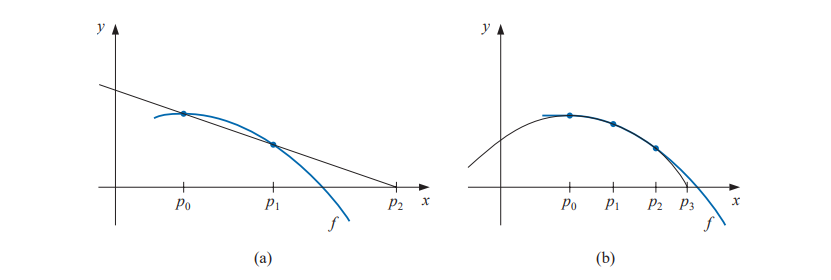
\includegraphics[width=1\linewidth]{figures/image.png}
    \caption{Minh họa hình học của phương pháp Müller}
    \label{fig:placeholder}
\end{figure}
\textbf{Ý tưởng.}  
Tại mỗi bước, ta tìm đa thức bậc hai nội suy $f(x)$ tại ba điểm gần nhau, rồi lấy giao điểm của parabol nội suy đó với trục $x$ làm điểm gần nghiệm kế tiếp.  
Công thức tổng quát của parabol nội suy có dạng:
\[
P(x) = a(x - p_2)^2 + b(x - p_2) + c,
\]
với $f_i = f(p_i)$.

Các hệ số $a,b,c$ được xác định bằng hiệu sai phân chia:
\[
\begin{aligned}
h_1 &= p_1 - p_0, \\
h_2 &= p_2 - p_1, \\
\delta_1 &= \frac{f_1 - f_0}{h_1}, \\
\delta_2 &= \frac{f_2 - f_1}{h_2}, \\
d &= \frac{\delta_2 - \delta_1}{h_2 + h_1}.
\end{aligned}
\]
Từ đó, ta có:
\[
a = d, \quad b = \delta_2 + h_2 d, \quad c = f_2.
\]

Giải phương trình $P(x) = 0$ cho ta nghiệm gần đúng mới:
\[
p_3 = p_2 - \frac{2c}{b \pm \sqrt{b^2 - 4ac}},
\]
trong đó dấu $\pm$ được chọn sao cho mẫu số có giá trị tuyệt đối lớn nhất (để tránh sai số trừ gần nhau):
\[
p_3 = p_2 - \frac{2c}{b + \operatorname{sgn}(b)\sqrt{b^2 - 4ac}}.
\]

Nếu $\Delta = b^2 - 4ac < 0$, phương pháp tự động sinh ra nghiệm phức, thể hiện khả năng xử lý nghiệm phức tự nhiên của nó.


\subsection{Thuật toán Müller (Müller’s Algorithm)}

\textbf{Các bước thực hiện:}
\begin{enumerate}
    \item Nhập $x_0, x_1, x_2$, sai số cho phép $TOL$, và số vòng lặp tối đa $N_0$.
    \item Với $i = 2, 3, \ldots, N_0$:
    \begin{align*}
        h_1 &= x_1 - x_0, & h_2 &= x_2 - x_1, \\
        \delta_1 &= \frac{f(x_1) - f(x_0)}{h_1}, & \delta_2 &= \frac{f(x_2) - f(x_1)}{h_2}, \\
        d &= \frac{\delta_2 - \delta_1}{h_2 + h_1}.
    \end{align*}
    Đặt $a = d$, $b = \delta_2 + h_2 d$, $c = f(x_2)$.
    \item Tính nghiệm gần đúng:
    \[
    x_3 = x_2 - \frac{2c}{b + \operatorname{sgn}(b)\sqrt{b^2 - 4ac}}.
    \]
    \item Nếu $|x_3 - x_2| < TOL$ hoặc $|f(x_3)| < TOL$, dừng lại.
    \item Ngược lại, đặt $x_0 = x_1, \; x_1 = x_2, \; x_2 = x_3$ và lặp lại.
\end{enumerate}

\textbf{Đặc điểm:}
\begin{itemize}
    \item Không cần đạo hàm của $f(x)$ như phương pháp Newton.
    \item Có thể tìm được nghiệm phức.
    \item Bậc hội tụ $\approx 1.84$ (nhanh hơn Secant, nhưng chậm hơn Newton).
    \item Cần ba giá trị khởi tạo ban đầu.
\end{itemize}

\textbf{Ví dụ 2.}  
Xét đa thức:
\[
f(x) = x^4 - 3x^3 + x^2 + x + 1.
\]
Chọn giá trị khởi tạo:
\[
x_0 = 0.5, \quad x_1 = -0.5, \quad x_2 = 0.
\]
Sau các bước lặp của phương pháp Müller, thu được:
\[
x_3 = -0.100000 + 0.888819i, \quad f(x_3) = -0.0112 + 3.0149i.
\]
Tiếp tục lặp, nghiệm hội tụ về:
\[
x \approx -0.339093 + 0.446630i.
\]
Do các hệ số của $f(x)$ là số thực, nên nghiệm liên hợp phức của nó cũng là nghiệm:
\[
\bar{x} = -0.339093 - 0.446630i.
\]
Nếu chọn các giá trị khởi tạo khác, chẳng hạn:
\[
x_0 = 1.5, \quad x_1 = 2.0, \quad x_2 = 2.5,
\]
thì phương pháp hội tụ đến nghiệm thực:
\[
x \approx 2.2888.
\]

\begin{figure}[H]
        \centering
        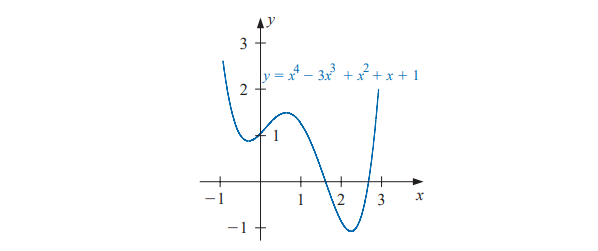
\includegraphics[width=1\linewidth]{figures/đt bậc 4.png}
        \caption{Đồ thị hàm số \[
f(x) = x^4 - 3x^3 + x^2 + x + 1.
\]}
    \label{fig:placeholder}
\end{figure}
        
\textbf{Nhận xét:}  
Phương pháp Müller có thể tìm được cả nghiệm thực và nghiệm phức của đa thức bậc cao, là một cải tiến đáng kể so với phương pháp Secant hoặc Newton khi xử lý các phương trình không có đạo hàm hoặc có nghiệm phức.

\textbf{Kết luận.}  
Phương pháp Müller là một sự mở rộng tự nhiên của phương pháp Secant, sử dụng nội suy bậc hai để xác định nghiệm gần đúng (có thể là phức) của phương trình phi tuyến.  
Với bậc hội tụ cao, không cần đạo hàm và khả năng phát hiện nghiệm phức, đây là công cụ mạnh trong việc tìm nghiệm của đa thức đại số bậc cao.  
Khi kết hợp với \textbf{kỹ thuật khử nghiệm (deflation)}, ta có thể lần lượt tìm được toàn bộ nghiệm của đa thức.


\section{Khử nghiệm của đa thức (Deflation of Polynomials)}

Sau khi tìm được một nghiệm của đa thức $P(x)$ (thực hoặc phức), ta thường muốn loại bỏ nghiệm đó để giảm bậc của đa thức và tiếp tục tìm các nghiệm còn lại.  
Quá trình loại bỏ nghiệm này được gọi là \textbf{deflation} (khử nghiệm hay khử bậc).

Giả sử $P(x)$ là đa thức bậc $n$ có dạng:
\[
P(x) = a_nx^n + a_{n-1}x^{n-1} + \cdots + a_1x + a_0,
\]
và ta đã tìm được nghiệm gần đúng $r$ của $P(x) = 0$. Khi đó, tồn tại một đa thức $Q(x)$ bậc $(n-1)$ sao cho:
\[
P(x) = (x - r)Q(x) + R,
\]
trong đó $R$ là phần dư. Nếu $r$ là nghiệm chính xác, thì $R = 0$.

\subsection{Khử nghiệm thực (Deflation for Real Roots)}

Để thực hiện phép chia này, ta sử dụng \textbf{phương pháp Horner} (Horner’s synthetic division).  
Ta viết:
\[
\begin{array}{r|rrrrr}
r & a_n & a_{n-1} & a_{n-2} & \cdots & a_0 \\ 
 &  & b_n & b_{n-1} & \cdots & b_1 \\ \hline
 & b_n & b_{n-1} & b_{n-2} & \cdots & b_0
\end{array}
\]
trong đó:
\[
\begin{aligned}
b_n &= a_n,\\
b_k &= a_k + r b_{k+1}, \quad k = n-1, n-2, \ldots, 0.
\end{aligned}
\]
Phần dư $R = b_0$, và các hệ số của đa thức thương $Q(x)$ là $b_n, b_{n-1}, \ldots, b_1$.  
Nếu $r$ chỉ là nghiệm gần đúng, ta có thể thực hiện \textit{một bước hiệu chỉnh} để cải thiện độ chính xác của $r$.

\textbf{Công thức hiệu chỉnh.}  
Giả sử sau khi khử nghiệm, ta được phần dư $R = P(r)$ và đa thức thương $Q(x)$.  
Theo Burden \& Faires, nghiệm $r$ có thể được hiệu chỉnh bằng công thức:
\[
r_{\text{new}} = r - \frac{R}{Q(r)}.
\]
Đây chính là \textit{một bước Newton} áp dụng cho hàm chia đa thức $(x - r)Q(x)$.

\textbf{Ví dụ 1.}  
Xét đa thức:
\[
P(x) = x^3 - 6x^2 + 11x - 6.
\]
Giả sử ta đã tìm được nghiệm $r = 1$.

Thực hiện Horner’s division:
\[
\begin{array}{r|rrrr}
1 & 1 & -6 & 11 & -6 \\ 
 &   & 1 & -5 & 6 \\ \hline
   & 1 & -5 & 6 & 0
\end{array}
\]
Đa thức thương là:
\[
Q(x) = x^2 - 5x + 6.
\]
Phần dư $R = 0$, chứng tỏ $x=1$ là nghiệm chính xác.  
Ta tiếp tục khử nghiệm trên $Q(x)$, ta được các nghiệm còn lại:
\[
x^2 - 5x + 6 = 0 \Rightarrow x = 2, 3.
\]

\subsection{Khử nghiệm phức (Deflation for Complex Roots)}

Khi nghiệm tìm được là \textbf{phức}, ví dụ $r = a + bi$ (với $b \ne 0$), thì nghiệm liên hợp $r^* = a - bi$ cũng là nghiệm (theo Định lý 2.20 trong sách):
\[
(x - r)(x - r^*) = x^2 - 2ax + (a^2 + b^2)
\]
là nhân tử bậc hai của $P(x)$.

Do đó, thay vì chia $P(x)$ cho $(x - r)$, ta thực hiện phép chia $P(x)$ cho \textbf{đa thức bậc hai thực}:
\[
x^2 - 2ax + (a^2 + b^2).
\]
Kết quả là một đa thức thực $Q(x)$ có bậc giảm 2, và phần dư $R(x)$ (nếu $r$ chỉ gần đúng) được dùng để hiệu chỉnh $a$ và $b$.

\textbf{Ví dụ 2.}  
Giả sử ta có đa thức:
\[
P(x) = x^4 - 3x^3 + x^2 + x + 1,
\]
và tìm được nghiệm gần đúng:
\[
r = -0.339093 + 0.446630i.
\]
Theo đó, nghiệm liên hợp là $r^* = -0.339093 - 0.446630i$.

Nhân tử bậc hai tương ứng:
\[
(x - r)(x - r^*) = x^2 - 2(-0.339093)x + [(-0.339093)^2 + (0.446630)^2] = x^2 + 0.678186x + 0.3125.
\]

Chia $P(x)$ cho nhân tử trên (dùng Horner mở rộng hoặc phép chia đa thức bậc hai) ta được:
\[
Q(x) = x^2 - 3.678186x + 3.200,
\]
với phần dư nhỏ (chứng tỏ nghiệm phức đã khá chính xác).

Giải $Q(x) = 0$ cho nghiệm thực còn lại:
\[
x = \frac{3.678186 \pm \sqrt{3.678186^2 - 4(3.200)}}{2} \Rightarrow x \approx 2.2888.
\]

\subsection{Phân tích và nhận xét}

\textbf{Đặc điểm.}
\begin{itemize}
    \item Deflation giúp giảm bậc của đa thức từng bước, nhờ đó dễ tìm các nghiệm còn lại.
    \item Với nghiệm thực, chỉ cần phép chia bậc 1 bằng Horner.
    \item Với nghiệm phức, cần chia bằng nhân tử bậc hai thực để tránh sai số phức không cần thiết.
    \item Khi nghiệm chỉ là gần đúng, việc deflation nhiều lần có thể tích luỹ sai số, vì vậy nên hiệu chỉnh lại nghiệm sau mỗi lần chia.
\end{itemize}

\textbf{Lưu ý quan trọng.}
\begin{itemize}
    \item Sau mỗi lần deflation, nên kiểm tra phần dư $R$ (hoặc $R(x)$) để đảm bảo nghiệm đủ chính xác.
    \item Nếu sai số còn lớn, áp dụng \textit{một hoặc vài bước Newton} trên đa thức gốc $P(x)$ để tinh chỉnh lại nghiệm.
    \item Khi tìm nghiệm phức, cần đảm bảo dùng biểu diễn số phức có độ chính xác kép để tránh làm tròn sai lệch giữa cặp liên hợp.
\end{itemize}

\textbf{Kết luận.}  
Phương pháp \textbf{deflation} là công cụ quan trọng giúp giảm bậc của đa thức sau khi tìm được một nghiệm (thực hoặc phức).  
Nó thường được sử dụng kết hợp với các thuật toán như \textbf{Müller’s Method} hoặc \textbf{Newton’s Method} để lần lượt xác định toàn bộ nghiệm của đa thức.  
Việc kiểm soát sai số và hiệu chỉnh nghiệm sau mỗi lần deflation là yếu tố then chốt đảm bảo độ chính xác của nghiệm cuối cùng.